
\documentclass[linenumbers,draft]{agujournal}
\journalname{Tectonics}
\usepackage{soul}
\usepackage{breakcites}
\usepackage[colorlinks = true,
            linkcolor = blue,
            urlcolor  = blue,
            citecolor = blue,
            anchorcolor = blue]{hyperref}

\begin{document}

\title{Late Holocene structural style and seismicity of highly transpressional faults in southern Haiti}

\authors{Jiannan Wang, Paul Mann, Robert R. Stewart}
\affiliation{}{Department of Earth and Atmospheric Sciences, University of Houston, Houston, Texas, USA.}

\correspondingauthor{Jiannan Wang}{jwang61@uh.edu}

\begin{keypoints}
\item First high-resolution sonar surveys of two actively deforming lakes in Haiti.
\item Extreme regional, tectonic transpression is partitioned by \textit{en~echelon} thrust faults and associated folds adjacent to a major strike-slip, plate boundary fault.
%\item Estimates of relative ages of deformation of major strike-slip faulting and \textit{en~echelon} thrusts from deformed and undeformed lake sediments.
\item 3D deformation model integrates patterns of 2010 coseismic uplift, aftershock distribution, and mapped geologic structures.
\end{keypoints}

\begin{abstract}
The devastating 2010 Haiti earthquake ($M_w$ 7.0) was caused by rupture of the L\'eog\^ane, blind, thrust fault located 5 km north of the 1200 km-long, left-lateral, Enriquillo-Plantain Garden fault zone (EPGFZ). Unexpectedly, the EPGFZ remained largely quiescent or slightly reactivated during the 2010 earthquake. Nevertheless, the EPGFZ still formed a major, crustal boundary between a coseismically-uplifted lowland north of the EPGFZ and a subsided area in the highlands south of the fault. Here, we use high-resolution sonar data from two, Haitian lakes that straddle the EPGFZ and its northern flank to demonstrate the presence of a 10 -- 15 km-wide, 120 km-long, late Holocene fold-thrust belt which deforms clastic, lowland basins along the northern edge of the EPGFZ. In the eastern part of the study area, sonar results from Lake Azuey show that the linear trace of the EPGFZ cutting the Holocene lake bed is more deeply buried and less active than the adjacent, newly discovered, northwest-striking, northeast-dipping Jimani thrust fault that is part of the adjacent, transpressional belt of \textit{en~echelon} thrusts and folds. This structural relationship between a less active EPGFZ and more recently active, transpression-related Jimani thrust is remarkably similar to the 2010 epicentral area 70 km to the west between the less active EPGFZ and seismogenic L\'eog\^ane thrust during the 2010 Haiti earthquake. In this complex transpressional zone, we propose that coseismic deformation alternates at recurrence intervals of centuries between oblique, transpression-related structures (L\'eog\^ane, Jimani, and Trois Baies thrusts) and the main strike-slip, plate boundary fault zone (EPGFZ).
\end{abstract}

\section{Tectonic setting of the 2010 Haiti earthquake}
\label{sec:intro}
On January 12, 2010, a $M_w$ 7.0 earthquake struck the densely populated, greater Port-au-Prince region of south-central Haiti and caused widespread destruction with over 230,000 fatalities and an estimated 10 billion dollars in damage \citep{prentice2010seismic,bilham2010lessons,paultre2013damage,kocel2016near} (Figure~\ref{figure1}). Multidisciplinary, geological and geophysical studies within the 2010 epicentral area of south-central Haiti include: 1) measurements and fault modeling of coseismic, coral reef uplift along a 50 km-long area of coastline in the epicentral region \citep{hayes2010complex}; 2) coseismic, vertical ground motion from radar interferometry \citep{hashimoto2011fan}; 3) high-resolution, surface-fault-trace mapping using Light Detection And Ranging (LIDAR) and targeted field studies \citep{cowgill2012interactive}; 4) Global Positioning System (GPS) and 2010 aftershock-based studies and modeling of pre-, syn-, and post-2010 earthquake crustal motions \citep{calais2010transpressional,nettles2010earthquake,symithe2013coseismic,douilly2013crustal,douilly2015three}; 5) ground-based studies of Holocene scarps including coseismic ground fractures and late Quaternary scarps of the EPGFZ that remained unaffected by 2010 fault breaks \citep{prentice2010seismic,koehler2011field,rathje2014geotechnical,saint2015seismotectonics}; 6) ground-based, near-surface, geophysical surveys of buried faults activated during the 2010 earthquake \citep{kocel2016near}; 7) near-coast surveys of submarine extensions of faults active in 2010 \citep{hornbach2010high,mercier20112010}; and 8) deepwater, marine surveys and coring to determine the recurrence interval of major earthquakes based on anomalous sedimentary deposits related to shaking and increased erosion \citep{mchugh2011offshore}. The consensus from these previous, on- and offshore, multidisciplinary studies is that the 2010 earthquake ruptured two, previously unrecognized west- to northwest-striking thrust faults located 2 to 5 km north of the 1200 km-long, left-lateral, Enriquillo-Plantain Garden fault zone (EPGFZ) that forms a major, plate boundary between the Caribbean plate to the south and the Gon\^ave microplate to the north \citep{mann1995actively,calais2010transpressional,benford2012gps,corbeau2016transpressive} (Figure~\ref{figure1}A, B). These two thrusts are separated by a distance of 6 km and include: 1) the subaerial, 8 km-long, blind, L\'eog\^ane thrust fault located 5 km north of the EPGFZ and trending at an angle of $8^{\circ}$ to the EPGFZ \citep{calais2010transpressional,douilly2013crustal,douilly2015three}; and 2) the submarine, 20 km-long Trois Baies thrust fault located 2 km north of the EPGFZ and trending at an angle of $20^{\circ}$ to the EPGFZ \citep{mercier20112010,symithe2013coseismic} (Figure~\ref{figure1}B, C).

Despite the proximity of the L\'eog\^ane and Trois Baies thrust to the neighboring EPGFZ, the EPGFZ remained largely quiescent and outside the zone of maximum, coseismic uplift and ground shaking and aftershocks produced by the 2010 earthquake \citep{nettles2010earthquake}. The centroid moment tensor (CMT) mechanism of the main 2010 shock shows a primarily strike-slip motion, with a small component of reverse motion, on a steeply north-dipping nodal plane \citep{nettles2010earthquake,douilly2013crustal}. Finite element modeling \citep{douilly2015three} suggests that L\'eog\^ane fault that is buried beneath at least 1 km of overlying undeformed clastic sediment in the area north of the EPGFZ absorbed northeast-southwest shortening related to extreme transpression along obliquely-striking, high-angle ($21^{\circ}$-$70^{\circ}$ dipping) reverse fault planes. For this reason, there was insufficient stress to trigger slip during the 2010 earthquake on the more east-west-striking EPGFZ located 5 km to the south (Figure \ref{figure1}B). Previous GPS surveys \citep{calais2010transpressional,calais2016plate} along this area of the EPGFZ have shown that plate motion is almost at right angles to these obliquely-striking thrusts and consistent with their preferred orientation for reactivation within the area of northeast-to-southwest shortening (Figure \ref{figure1}A, B).

Aftershock studies following the 2010 earthquake by \citet{douilly2013crustal,douilly2015three} showed that the EPGFZ moved locally at depth and acted as a 6 km-long, east-west and sub-vertical, connecting fault segment that transmitted seismogenic motion between the obliquely-trending, north-dipping, L\'eog\^ane fault in the east and the more obliquely-trending, southwest-dipping Trois Baies fault in the west (Figure \ref{figure1}B). However, post-earthquake geologic reconnaissance revealed no fault-related, surface ground breaks along the proposed onland areas of EPGFZ in the epicentral region of the earthquake \citep{prentice2010seismic,koehler2011field,rathje2014geotechnical}. A more recent study by \citet{saint2015seismotectonics} proposed previously, unrecognized, 2010 coseismic groundbreaks along the obliquely-trending Lamentin thrust 11 km east of the epicentral area near the city of Port-au-Prince (Figure \ref{figure2}A).

\textit{En~echelon} thrusts spacing at distances of 1-8 km along the main strike-slip fault, obliquely intersect the main strike-slip fault at angles of $30^{\circ}$ -- $45^{\circ}$. These structures strike northwestward away from the EPGFZ for distances of 4-29 km into the more thickly-sedimented basinal areas north of the EPGFZ (Figure~\ref{figure2}A).  As a result of this distinctive and regular intersecting fault geometry between these oblique thrusts and the linear EPGFZ, earthquake rupture initiating on an oblique thrust, as seen for the L\'eog\^ane fault in 2010, is likely confined to that northern area vicinity and may not connect with other oblique thrusts or even the EPGFZ itself \citep{douilly2013crustal,douilly2015three}.

Coseismic deformation along a large transpressional strike-slip fault, such as the EPGFZ \citep{calais2002strain} in Hispaniola or the San Andreas fault zone in California \citep{segall1990surface}, is either accommodated by: 1) slip and major earthquakes on the main, strike-slip plate boundary fault; 2) the oblique, \textit{en~echelon} thrusts adjacent to the main fault; 3) or both sets of faults (cf. compilation of types of destructive earthquakes in transpressional settings by \citet{hayes2010complex}). Motions on distributed, \textit{en~echelon} thrusts do not necessarily spare or reduce coseismic rupture on the main strike-slip fault because the \textit{en~echelon} and main strike-slip fault remain separate fault planes, and the main strike-slip fault would continue to accumulate strain. In an extreme transpression case as observed in Haiti, plate motions become increasingly convergent across the main, strike-slip fault zone (Figure~\ref{figure1}A, B). In such a setting, the \textit{en~echelon}, oblique thrusts might assume more and more plate-edge strain to the point that the plate boundary behaves more like a broad, thrust boundary and less like a narrow, strike-slip boundary \citep{mount1987state}.

These oblique and \textit{en~echelon} thrust faults in transpressional settings, that includes large restraining bends such as Hispaniola, potentially nucleate ``uncharacteristic earthquakes'' of varying recurrence intervals and sizes that are distinct from the recurrence intervals and sizes of the adjacent but independent strike-slip faults \citep{Fielding2013}. Restraining bend areas like Hispaniola can lead to the generation and increased activities on more favorably and obliquely oriented folds and thrusts whose coseismic rupture might alternate with much longer ruptures along the adjacent strike-slip fault. The number of these \textit{en~echelon} thrust faults can be large at observed spacings of 5-10 km dispersed along the trend of strike-slip faults that may be hundreds of kilometers in total length. For this reason, the identification and earthquake potential of oblique \textit{en~echelon} thrusts, especially when buried or ``blind'', can be challenging to assess in transpressional zones \citep{frankel2011seismic}.

\section{Objectives and methods}
\subsection{Study area}
The elongate, belt of transpressional deformation associated with \textit{en~echelon} thrusts occupies a topographically-low, densely populated Cul-de-Sac basin underlain by poorly-consolidated, clastic sedimentary rocks ranging in age from Miocene to Recent \citep{massoni1955haiti,mann1995actively,terrier2014revision,saint2015seismotectonics}. In easternmost Haiti, this belt is overlain by the shallow (33 m-deep), 138 km\textsuperscript{2}, brackish Lake Azuey near the border separating Haiti from the Dominican Republic \citep{wright2015factors,piasecki2016bathymetric}. Lake Enriquillo to the east is twice as large (346 km \textsuperscript{2}) as Azuey, shallow (52 m-deep), hypersaline, about 40 m below sealevel, and located entirely in the Dominican Republic. Lake Enriquillo is separated from Lake Azuey by the eastward continuation of the same transpressional belt parallel and north of the EPGFZ in the Cul-de-Sac valley \citep{mann1995actively} (Figure \ref{figure1}B). 

In the western part of our study area, the more transtensional segment of the EPGFZ is overlain by the 42.8 m-deep, 14 km\textsuperscript{2}, freshwater Lake Mirago\^ane (Figure \ref{figure1}B). All three of these shallow, inland, lakes experience variations up to 13 m in their surface elevations due to annual to decadal changes in climate and rainfall amounts including extreme rainfall events associated with hurricanes \citep{wright2015factors,piasecki2016bathymetric,moknatian2017development,rico2017hydrodynamic}.  

\subsection{Objectives}
The main goal of this paper is to better integrate the geologic structure of the 120 km-long study area, which parallels the trace of the EPGFZ and includes the 2010 epicentral area. Data types that we have integrated for this study include: surficial-geologic mapping, geophysics, GPS, radar interferometry, aftershocks, and modeling studies. Most of these studies were completed in the aftermath of the 2010 earthquake. Our study integrates these datasets in order to structurally characterize the 10-15 km-wide, belt of late Holocene, transpressional deformation that forms a laterally-extensive, deformed belt along the inland, Cul-de-Sac intermontane basin in the east and the low-relief coastal plain along Port-au-Prince bay and the Canal du Sud to the west (Figure~\ref{figure1}B). In particular, we focus on the identifying a family of \textit{en~echelon} thrusts, whose curvilinear strikes area are very similar to the L\'eog\^ane thrust now known to be responsible for most of the energy release and coseismic uplift during the 2010 Haiti earthquake \citep{calais2010transpressional,douilly2013crustal,douilly2015three} (Figure \ref{figure1}B, Figure \ref{figure2}A).

\subsection{Survey design}
In order to understand the geologic and structural styles of transpression within this belt, including the age relations between deformation in the north-flanking belt and the EPGFZ itself, we collected a total of 94 km of high-resolution (2-10 kHz) sonar profiles in 2014 from the 138 km\textsuperscript{2}, brackish Lake Azuey and 37 km of profiles from the 14 km\textsuperscript{2}, fresh-water Lake Mirago\^ane (Figure~\ref{figure1}B). The EPGFZ strikes through both of the lakes, so 80\% of our lines on Lake Azuey and 90\% of our survey lines on Lake Mirago\^ane were dedicated to the across fault-strike, north-south profiles. 

The average speed of the small, outboard, motorboat towing the sonar was 3 knots, with a sonar pulse rate of 4 per second. Our 2-10 kHz sonar frequency range yielded sub-bottom layer resolution of about 10 cm \citep{wang2015inferring}. These surveys were the first sonar surveys in Haitian lakes. Both lakes straddle the projected active trace of Haiti's EPGFZ and its adjacent, transpressional fold-thrust belt, and therefore provide new constraints on the location, structural style, and timing of deformation within both structural provinces. We integrate these lake data with previous geologic mapping, geophysical observations related to the 2010 earthquake, and regional information on plate motions in this region. 

\section{Tectonic setting of transpressional deformation in south-central Haiti including unresolved tectonic and structural questions}
\label{sec:tectonic}
\subsection{Previous strike-slip deformational model vs. Haiti thrust belt deformational model}
There are two, previously-proposed, regional structural models to explain the present-day structure of the broad, 250 km-wide zone of transpression spanning the entire width of the island of Hispaniola.

\subsubsection{Strike-slip, regional structural model}
The first is the strike-slip-dominated model, driven by oblique motion and transpression between the thick and buoyant Bahamas platform on the North America plate, the Caribbean plate, and the Gon\^ave microplate \citep{mann1995actively,dolan1998active,mann2002oblique,calais2002strain,calais2016plate} (Figure~\ref{figure1}A, B). GPS surveys within this 250 km-wide, transpressional zone \citep{calais2002strain,calais2010transpressional,hayes2010complex,symithe2013coseismic,douilly2013crustal,douilly2015three} reveal strain partitioning along the EPGFZ and the subparallel Septentrional strike-slip fault zone 200 km to the north (which is the plate boundary separating the North Hispaniola microplate and Gon\^ave microplate) (Figure {\ref{figure1}}A). As a result of this oblique collision and restraining bend area, the 3-km-high mountains of central Hispaniola have grown since the late Miocene to an elevation of 3 km to the highest range in the northern Caribbean. 

The left-lateral strike-slip rupture of the EPGFZ in the 18th century inferred from the map pattern of historical earthquakes \citep{bakun2012significant} combined with average late Holocene, left-lateral offset amounts of 1.3 -- 3.3 m as expressed along offset streams of the EPGFZ \citep{prentice2010seismic} and by late Holocene, left-lateral, channel offsets of 7 -- 8 m along stream channels offset by the Septentrional fault zone \citep{prentice1993paleoseismicity,prentice2003slip}. 

The study by \citet{saint2015seismotectonics} indicates that the folding and thrusting of 10 -- 15 km-wide belt of Miocene to Quaternary rock was generated by transpression along the EPGFZ. In addition, \citet{mann2002oblique,grindlay2005high,kroehler2011late} suggest a strong, southwestward, backthrusting of the southern Hispaniola in Haiti and Dominican Republic to the southwest onto the Caribbean plate (Figure \ref{figure1}B, C). Southwestward backthrusting of Hispaniola is manifested by the large accretionary wedge along the Muerto trench south of the Dominican Republic \citep{bien1986contribution,bruna2009morphotectonics} (Figure \ref{figure1}A, B) and along the southern margin of Haiti (South Haiti accretionary prism \citep{bien1986contribution} (Figure \ref{figure1}C). A localized, negative gravity anomaly marks the trend of plate flexure of the underthrusting Caribbean plate beneath the overriding area of southern Hispaniola \citep{mann2002oblique,bruna2009morphotectonics} (Figure \ref{figure1}A)).

\subsubsection{Criticisms of the strike-slip, regional structural model}
Two criticisms have been proposed for the strike-slip model. First, \citet{corbeau2016transpressive} noted that the predictions of the GPS-based block models overestimate the observed amounts of transpression-related shortening seen on seismic reflection profiles in the offshore area of the Gulf of Gon\^ave north of the southern peninsula of Haiti, or in the area of the Jamaica Passage east of Haiti. Second, \citet{symithe2016present} have proposed that there is no geologic evidence for a continuation of the EPGFZ east of latitude $72.27^{\circ}$W in the eastern Cul-de-Sac Valley, Lake Azuey and Lake Enriquillo in the Dominican Republic (Figure~\ref{figure1}B). Instead, \citet{symithe2016present} propose that the high rates of north-south shortening predicted from GPS block models are accommodated entirely by low-angle thrust structures in the eastern Cul-de-Sac and Enriquillo Valleys that were modeled using GPS data as part of their study.

\subsubsection{Trans-Haitian fold-and-thrust belt regional structural model}
The Trans-Haitian fold-and-thrust belt model originated with a study by \citet{pubellier2000plate}, who proposed a low-angle southwestward-verging fold-and-thrust belt along the southwestern edge of the central Hispaniola block. The thrust front of this feature was thought to be actively propagating from the main Trans-Haitian fold-and-thrust belt, that is located in the Cha\^ine des Matheux (Figure~\ref{figure1}B, Figure~\ref{figure2}A), southwestward into the area of the L\'eog\^ane plain and the Cul-de-Sac basin (Figure \ref{figure2}A, B). \citet{pubellier2000plate} proposed that the EPGFZ originally formed as a left-lateral strike-slip fault, but became inactive in the late Miocene when deformation in southern Hispaniola became inactive. Increasing amounts of shortening caused the Trans-Haitian fold-and-thrust belt to propagate into the southern area of the Cul-de-Sac basin and L\'eog\^ane plain, where it emerged or ``daylighted'' to form the \textit{en~echelon}, convergent structures (compiled on the map in Figure \ref{figure2}). \citet{pubellier2000plate} also proposed that the EPGFZ was reactivated as a normal fault in the Quaternary as a result of crustal loading of the southern, foreland area by the overthrusting Trans-Haitian fold-and-thrust belt. 

Following the 2010 earthquake and the recognition of the north-dipping blind L\'eog\^ane thrust fault, \citet{calais2010transpressional} proposed that the L\'eog\^ane fault marks the leading edge of the Trans-Haitian fold-and-thrust belt rather than being an \textit{en~echelon} thrust genetically linked to the EGPFZ. In the interpretation proposed by \citet{calais2010transpressional}, the northward dip of the L\'eog\^ane thrust made it difficult to link its origin with the EPGFZ, whose dip had been established in this area as a vertical to high angle (> $60^{\circ}$), south-dipping fault plane with evidence of late Holocene, left-lateral offsets of drainages \citep{prentice2010seismic}. Moreover, \citet{symithe2016present} noted that Trans-Haitian fold-and-thrust belt regional model of \citet{pubellier2000plate} was more consistent with GPS data showing larger magnitude, north-south shortening in central Hispaniola than with the existence of an eastward extension of the left-lateral EPGFZ into the eastern part of Haiti and the Dominican Republic (Figure~\ref{figure1}B and Figure~\ref{figure2}A).

\subsubsection{Criticisms of the Trans-Haitian fold-and-thrust belt, regional structural model}
First, \citet{mercier20112010} pointed out two problems with linking the origin of the L\'eog\^ane thrust to the southwestward-propagating edge of the Trans-Haitian fold-and-thrust belt: 1) the dip of the fault generating the main thrust, as imaged by \citet{mercier20112010}, was more steeply dipping ($64^{\circ}$) than expected for a blind thrust at the leading edge of a fold-thrust belt; and 2) the orientation of the N$84^{\circ}$E fault plane of the main shock is significantly oblique to the N$120^{\circ}$E-oriented leading edge of the Trans-Haitian fold-and-thrust belt as proposed by \citet{pubellier2000plate}. In this paper, we discuss other inconsistencies with the previous interpretation that deformation north of the EPGFZ is the result of southwestward propagation of the Trans-Haitian fold-and-thrust belt.

\section{New observations of the Late Holocene structural style along EPGFZ in southern Haiti}
\subsection{Significance of \textit{en~echelon} thrusting and folding north and south of the EPGFZ}
The presence of a strike-slip fault at any scale is indicated by the presence of \textit{en~echelon} arrays of thrust faults, normal faults, folds, fractures, dikes, and other linear features in narrow, elongate zones \citep{sylvester1988strike}. On Figure~\ref{figure2}A, we have compiled geologic information on \textit{en~echelon} folds and faults in a 10 -- 15 km-wide zone of deformation along both the northern and southern flanks of the EPGFZ. Folds form as fault propagation folds along oblique, thrust faults, vary from 1 to 8 km in lateral spacing, and deform Miocene and younger fine to coarse-grained, basinal, and coastal plain rocks in the belt that is 10 -- 15 km wide and extends parallel to the EPGFZ for 120 km (Figure~\ref{figure1}B and Figure~\ref{figure2}A). Folds in Neogene clastic lithologies of the Cul-de-Sac basin contrast with more continuous and longer wavelength, \textit{en~echelon} fold axes present in more massively-bedded Cretaceous to Eocene rigid, basaltic, and carbonate lithologies exposed in the 2 km-high range south of the EPGFZ, the Massif de Selle (Figure~\ref{figure2}A). The curvilinear trend of fold axes is similar both to the north and south of the EPGFZ and indicates a genetic relation between left-lateral shearing along that fault and the formation of those \textit{en~echelon} features (Figure~\ref{figure2}B). 

The \textit{en~echelon} distribution of complex Holocene folding and thrusting in the 10 -- 15 km wide zone of deformation north of the EPGFZ is also reflected in the complex pattern of 2010 coseismic and vertical deformation recorded by the interferogram from the 2010 epicentral area on the L\'eog\^ane plain west of the Cul-de-Sac basin \citep{hayes2010complex,hashimoto2011fan,bilham2013remote} (Figure~\ref{figure2}A). \citet{douilly2013crustal,douilly2015three} and \citet{kocel2016near} use aftershocks and shallow geophysics to show that the 2010 L\'eog\^ane thrust fault and sub-parallel faults are overlain by at least one kilometer of undeformed and sub-horizontal strata (cross-section A--A' in Figure~\ref{figure3}).

\subsection{Significance of curvilinear fold and thrust patterns in the transpressional belt north of the EPGFZ}
The shaded relief DEM (digital elevation model) shown in Figure~\ref{figure2}B reveals the curvilinear, \textit{en~echelon} fold morphologies that are defined by low, bedrock hills of Neogene sedimentary rocks exposed on the flat-lying Cul-de-Sac basin. These curvilinear fold axes can be related directly to a broad zone of left-lateral, simple shear produced along the sub-vertical and left-lateral EPGFZ based on several, basic observations seen on Figure~\ref{figure2}B. The most prominent folds present along the southern edge of the Cul-de-Sac basin are within 15 km of the EPGFZ. In contrast, the central and northern edges of the Cul-de-Sac basin exhibit no prominent folding, even directly adjacent to the base of Eocene-Miocene carbonate rocks forming the range \citep{pubellier2000plate} (Figure~\ref{figure2}A). The mapview shapes of fold axes along the southern margin of the Cul-de-Sac basin are asymptotic, or gently curve into east-west parallelism with the main trace of the EPGFZ along the southern edge of the Cul-de-Sac basin, as observed in claybox experiments of shearing (see the inset of Figure~{\ref{figure2}}B; modified from \citet{odonne1983analogue}). Deeper, structural depressions form in the zone of convergent intersection between the east-west-striking EPGFZ and the northwest-striking, secondary thrusts as seen in the southern part of Lake Azuey, where the lake bends from an east-west trend adjacent to the EPGFZ to a more northwest trend in the central and northern part of the basin (Figure~\ref{figure2}A, B).

\subsection{Geologic structure of the area of \textit{en~echelon} thrusts in the epicentral area on the L\'eog\^ane fan-delta}
\subsubsection{Geologic structure of the L\'eog\^ane fan area}
A cross-sectional profile of the 2010 epicentral area related to the activation of two conjugate thrust faults is modified from aftershock data from \citet{douilly2013crustal,douilly2015three} and is shown in Figure~\ref{figure3} (Line A--A'). Both faults are buried by about 1 km of late Quaternary sand and gravel of the L\'eog\^ane fan delta \citep{kocel2016near} and an additional 1 km of Paleocene limestone. Aftershocks indicate that the main thrust event ruptured a depth range of from 4 to 17 km beneath the ground surface \citep{douilly2013crustal,douilly2015three}. The orientation of the L\'eog\^ane thrust based on gravity and uplift of coastal features is east-west and parallel to recent near-surface breaks of the EPGFZ mapped in the shallow, coastal zone adjacent to the L\'eog\^ane plain \citep{hornbach2010high}. Due to its proximity to the EPGFZ, an east-west strike of the L\'eog\^ane thrust is predicted as this is the area where \textit{en~echelon} folds and faults curve into an asymptotic orientation relative to the main EPGFZ, as shown on Figure~\ref{figure2}B.

A radar interferogram compiled on the structure map of Figure~\ref{figure2}A revealed that the 2010 earthquake elevated the smaller folds of the L\'eog\^ane fan-delta north of the EPGFZ, yet produced coseismic subsidence in the 1.4 km-high, less complexly deformed, mountain range south of the EPGFZ \citep{hashimoto2011fan} (Figure~\ref{figure2}A). This paradox can be simply explained by the northward dip of the seismogenic L\'eog\^ane fault that elevated the basinal area to the north (hanging wall of the L\'eog\^ane fault) and depressed the mountainous area to the south (footwall block of the L\'eog\^ane fault (line A--A' in Figure~\ref{figure3}). 

\subsubsection{Geologic structure of the Port-au-Prince urban area compared to the L\'eog\^ane epicentral area} 
A similar pattern of deformation is observed in Port-au-Prince urban area where the central and northern edge of the Cul-de-Sac basin is only gently folded and faulted \citep{massoni1955haiti,cox2011shear,mchugh2011offshore,saint2015seismotectonics} (Line B-B' in Figure~\ref{figure3}). The cross section taken from workers, who were mapping 60 years ago when Port-au-Prince was smaller and the geology was less obscured by urbanization, shows two large thrusts, a range-bounding thrust along the southern edge of the city, and a northeast-dipping thrust, the Dumay thrust, that elevates a broad outcrop zone of north-dipping, Neogene sedimentary rocks on which the northern area of Port-au-Prince is built \citep{rathje2014geotechnical}. The $50^{\circ}$ northeast dip of the Dumay thrust is similar to the $70^{\circ}$ northeast dip of the L\'eog\^ane thrust to the west known from aftershocks \citep{douilly2013crustal,douilly2015three}, although the dip of the Dumay thrust reverses to a southwest dip as it approaches the EPGFZ (Figure~\ref{figure2}A, B). 

On the cross section B--B' in Figure~\ref{figure3}, we have indicated areas that are elevated as a result of the northward dip of the Dumay thrust and the depression of the area to the south of the EPGFZ in the highlands south of the EPGFZ. If a future earthquake occurred along the north-dipping, \textit{en~echelon} thrust faults in the Port-au-Prince area (Line B--B' in Figure~\ref{figure2}) or Lake Azuey area (Line C--C' in Figure~\ref{figure2}) a similar uplift phenomenon is likely to occur where the lowlands north of the EPGFZ are uplifted and the adjacent mountains south of the EPGFZ subside.

\subsubsection{Geologic structure of the Lake Azuey area} 
In the Lake Azuey area, we mapped a linear, 250--500 m-wide, and east-west striking fault trace in deformed Holocene sediments along the projected trend of the landward traces of the EPGFZ both east and west of Lake Azuey (Figure~\ref{figure4} and Figure~\ref{figure5}A -- D). The fault is marked by a 250--500 m-wide, graben-like feature that disrupts the uppermost late Holocene, lake stratigraphy. Integrated with previous land mapping of the EPGFZ \citep{bourgueil1988synthese,mann1995actively,prentice2010seismic,cowgill2012interactive}, we interpret this linear east-west striking feature in Lake Azuey as a 250--500 m-wide and continuous trace of the EPGFZ which we can follow westward to the EPGFZ locality at Dumay, about half way between Lake Azuey and Port-au-Prince, which was previously described and dated as a 6 m-long, left-lateral offset of a late Holocene stream channel \citep{cowgill2012interactive} (locates at red circle, which is labeled as Dumay in Figure~\ref{figure2}A). A similar, 500 m-wide, graben-like structure was described by \citet{hornbach2010high} along the trace of EPGFZ where it enters the Baie de Grand Go\^ave 75 km west of Lake Azuey (Figure~\ref{figure2}A). 

The structural cross sections in this area were compiled from previous studies \citep{massoni1955haiti,mann1995actively,douilly2015three} and indicate that the high-angle EPGFZ co-exists with the adjacent thrusts that over-thrust from the south and north (Line B--B' in Figure~\ref{figure3}). We project this trace of the EPGFZ along a prominent fault valley at the town of Jimani that separates Lakes Azuey and Enriquillo (Figure~\ref{figure2}A and Figure~\ref{figure4}). Sonar profiles (Figure~\ref{figure5}A -- D) show that the most recent rupture of the EPGFZ is covered by about 0.7 m of Holocene sediment, suggesting that there has been late Holocene activity of the EPGFZ along the southern edge of the lake.

From sonar data, we observed late Holocene lake sediments onlapping onto local highs of Eocene limestone of the bounding range along the northern edge of the EPGFZ, indicating that this margin is not controlled by late Holocene faulting (Figure~\ref{figure5}C, E). The sonar from southern Lake Azuey suggests that the most prominent folds present adjacent to the EPGFZ become less prominent in the central and northern parts of the lake (Figure~\ref{figure2}B). These southern folds and thrusts imaged in Lake Azuey define the transpressive belt along the EPGFZ observed in onshore areas to the west. On the cross section in Figure~\ref{figure5}E, we have schematically indicated areas that are elevated as a result of the northward dip of the Jimani thrust and the depression of the area to the south of the EPGFZ.

The structural cross-section (Figure~\ref{figure5}E) of the Lake Azuey area and the previous works \citep{massoni1955haiti,bourgueil1988synthese,cox2011shear,douilly2015three} (Line A--A' and B--B' in Figure~\ref{figure3}) along this 120 km-long zone of deformation adjacent to the EPGFZ show that the oblique thrust faults share a similar orientation with other northeast-dipping thrusts along the northern edge of the EPGFZ. All three of these oblique thrust faults (the L\'eog\^ane thrust in Line A--A', the Dumay thrust in Line B--B', and the Jimani thrust in Figure~\ref{figure5}E) shown on the cross sections deform rocks as young as Pliocene and Quaternary \citep{saint2015seismotectonics}. 

On a more regional scale, these observations from Lake Azuey are consistent with the multi-channel seismic reflection profile (named as Canadian Superior 2D and shown in Figure~\ref{figure1}C), that shows a lack of intensive deformation in the part of Port-au-Prince Bay, that is the offshore, largely un-faulted and folded seaward extension of the Cul-de-Sac basin \citep{mchugh2011offshore}. \citet{pubellier2000plate} proposes that the Trans-Haitian fold-and-thrust belt exposed in the Chaine des Matheux range extends beneath the entire Cul-de-Sac and Port-au-Prince basins (Figure~\ref{figure2}A, B). In summary, our observations at this scale do not support the previous model by \citet{pubellier2000plate} and \citet{calais2010transpressional} that folds and faults of the northern range are propagating southwestward beneath the zone of \textit{en~echelon} faults and folds (Figure~\ref{figure2}A, B).

\subsection{Subsurface stratigraphy of Lake Azuey and Lake Enriquillo and paleoseismic estimates of the relative timing of recent earthquakes on the EPGFZ and secondary, \textit{en~echelon} thrust faults}
Our objective is to determine the relative age of the EPGFZ and its adjacent zone of fold-and-thrust deformation using the sonar profiles from Lakes Azuey and Enriquillo (Figure~\ref{figure6}A). Previous coring, both in Lake Enriquillo \citep{rios2013holocene} (which was tied to the onshore stratigraphic studies \citep{taylor1985stratigraphy,rios2013holocene}) and in Lake Mirago\^ane \citep{higuera199910}, has established the late Holocene history in the upper 5 m and 7 m sediment, respectively.

In Lake Enriquillo, a sonar survey similar to ours was conducted in 2013 \citep{rios2013holocene}. Mapping in both lakes revealed the presence of the east-west, sub-parallel strands of the EPGFZ that are collinear with onland scarps both east and west of Lake Azuey (Figure~\ref{figure2} and Figure~\ref{figure4}) and east and west of Lake Enriquillo \citep{mann1995actively,rios2013holocene} (Figure~\ref{figure6}A). These east-west fault strands abruptly truncate the trends of folds in the ranges south of the lake (Figure~\ref{figure4}). The sonar events, which are interpreted as stratigraphic features, from Lake Azuey and Lake Enriquillo (Line B1 and Line L19 correlate convincingly (Figure~\ref{figure6}B). \citet{schwartz1980herpetogeography} suggested that both of the lakes were the results of the closure of former marine strait. Due to the small distance separating the two lakes (about 4 km), the two lakes merged during heavy rainfall years \citep{greer2006decadal,medley2007paleosalinity,romero2011water}. Given the similarity of the stratigraphic profiles, and the same amount of sediment above the EPGFZ, it is reasonable to suggest that Lake Azuey and Lake Enriquillo share the similar sedimentation history as well as the same structural style and seismicity related to the EPGFZ and its oblique, thrust faults. However, this hypothesis remains speculative pending more coring in Lake Azuey.

The EPGFZ in both Lake Enriquillo and Lake Azuey is buried by 0.7 m of sediments. According to coring studies in the Dominican Republic \citep{taylor1985stratigraphy,rios2013holocene}, the 5.2 m thickness of the latest lake stage (2 ka BP to present) gives a recent Holocene average sedimentation rate of 2.6 mm/yr (Figure~\ref{figure6}B). Using the average sediment rate, the most recent rupture of the EPGFZ would be dated to some 270 years ago. Given the historical earthquake records \citep{bakun2012significant}, we suggest that the most recent rupture of the EPGFZ corresponds to the historical events of October or November 1751 (267 years ago), and that the deformed sediments in Lake Azuey are of Holocene age \citep{rios2013holocene}.

\subsection{Easternmost extent of the EPGFZ trace in Lake Enriquillo, Dominican Republic}
Based on both of our lake surveys combined with a previous survey of Lake Enriquillo in the Dominican Republic \citep{rios2013holocene}, and the previous geologic mapping of the basinal and topographic corridor of the Cul-de-Sac basin in Haiti and the Enriquillo basin in the Dominican Republic \citep{mann1995actively,mann1999caribbean}, a basic question we pose is whether the EPGFZ extends as a continuous, strike-slip fault along the 120 km-long zone of deformation of Miocene and younger clastic rocks present between the two lakes (Figure~\ref{figure1}B and Figure~\ref{figure6}A). Previous studies \citep{saint2015seismotectonics,symithe2016present} have proposed that the EPGFZ terminates as a strike-slip feature in the area south of Port-au-Prince. These studies further have proposed that transpressional plate motion in the eastern Cul-de-Sac basin and the Enriquillo Valley in the Dominican Republic (Figure~\ref{figure1}B and Figure~\ref{figure6}A) is entirely accommodated along the low-angle oblique-thrust structures that overthrust the southern edges of Lake Azuey and Lake Enriquillo. 

A previous study of Lake Enriquillo by \citet{rios2013holocene} identified the break along the northeastern edge of Cabritos Island in Lake Enriquillo, which aligns exactly with the prominent, east-western lineament extending eastward from our map area in Lake Azuey (Figure~\ref{figure6}A). The sonar results from both lakes show that the EPGFZ extends to at least to the eastern tip of Cabritos Island in the center of Lake Enriquillo, Dominican Republic (Figure~\ref{figure6}A). This survey revealed a fault penetrating the youngest sediment layer of Holocene age which is consistent with recent activity on this segment of the EPGFZ (Figure~\ref{figure5}A -- D). Therefore, we conclude that this linear, late Holocene strike-slip fault extends at 55 km (at least) to the eastern edge of Lake Enriquillo, where the previously documented \citep{mann1995actively} uplift of the Holocene reef fringes Lake Enriquillo.

\section{Active tectonics of the area west of the 2010 epicentral zone in the western study area: L\'eog\^ane plain, Mirago\^ane basin, and their adjacent offshore area}
\subsection{The Trois Baies thrust fault, Canal du Sud, as the termination structure for the 2010 earthquake}
The 2010 aftershock zone at the western and central part of our study area (Figure~\ref{figure7}A) reflects the rupture along the northwest-striking, 20 km-long, submarine, Trois Baies thrust fault that forms the western extension of the 10 -- 15 km-wide, transpressional zone north of the EPGFZ \citep{mercier20112010}. As the Trois Baies fault is is a submarine fault, InSAR cannot be used to assess its 2010 coseismic similarity with folding and thrusting along the L\'eog\^ane thrust that affected the onshore, L\'eog\^ane plain (Figure~\ref{figure7}A). 

Nevertheless, the same basic structural elements of the L\'eog\^ane plain are also observed for the offshore Trois Baies thrust fault, which include its proximity (1 km) to the EPGFZ and its steep ($45^{\circ}$) but opposite (southwest) dip of the Trois Baies thrust fault (Figure~\ref{figure7}). One of the most intense zones of 2010 coseismic, aftershock, coastal uplift \citep{hashimoto2011fan}, and subsidence \citep{prentice2010seismic} separates the oppositely-dipping L\'eog\^ane and Trois Baies faults, and may represent complex deformation at a transfer zone between the two, oppositely-dipping thrust faults (Figure~\ref{figure7}A, B). The aftershock study of the Trois Baies fault \citep{symithe2016present} shows that its thrust character and oblique orientation in map view with the main EPGFZ is comparable to the cross sections of the eastern area in Figure~\ref{figure3}. In the map view, the overall structure of this western part of the study area mirrors the same geometrical relationship between the oblique thrusts (such as the Trois Baies thrust fault) and the main EPGFZ as described at the eastern part of the study area (Figure~\ref{figure2}).

\subsection{Structure of the Mirago\^ane pull-apart basin}
In the onshore part of the western study area, Lake Mirago\^ane was interpreted as a 14 km\textsuperscript{2} pull-part basin developed as a left-stepping, releasing bend on the EPGFZ paired with the adjacent Tapion du Petit Go\^ave restraining bend 12 km to the east (Figure~\ref{figure7}) \citep{mann1995actively,cowgill2012interactive}. Bathymetry from our sonar data shows the maximum water depth of Lake Mirago\^ane is 42.8 m (Figure~\ref{figure7}B), which makes this lake the deepest \citep{higuera199910} in the entire Caribbean region. The 30 m of recognizable stratigraphy (Figure \ref{figure8}B and C) from the sonar survey in Lake Mirago\^ane reveals a series of deformational features including major east-west normal faults, minor thrust faults at depth (some 20 m), and active folds at the lake bottom (Figure~\ref{figure8}). The upper 7 m of the lake sediments were cored and dated at 10 ka at the bottom of the core \citep{higuera199910}. By applying the average sedimentary rate from the core data to the chirp sonar trace, we can extrapolate the sedimentation rate to the observed thickness of 30 m in the lake and estimate a minimum of 43 ka for the age of formation for the pull-apart basin along the EPGFZ. Core measurements of the E/P (evaporation and precipitation ratio from the $\delta^{18}$O of ostracod shells in the core sample) were carried out \citep{higuera199910} (Figure~\ref{figure9}B). The core reveals that the uppermost part of the sediments are Holocene to the latest Pleistocene in age (Figure~\ref{figure9}A). Pollen data from the core indicate alternating dry and wet environments.

\subsection{Ages and sedimentary cycles of the Mirago\^ane pull-apart basin}
We applied a low-pass filter on the pollen log data (from the core acquired by \citet{higuera199910} in the center of the lake) and found a strong correlation between the pollen and sonar data (red curve in Figure~\ref{figure9}B). To further investigate this interesting correlation between the paleoenvironmental and geophysical data, we use the filtered E/P log, considered as pseudo-acoustic impedance log, to generate a synthetic sonar response (Figure~\ref{figure9}B). The correlation suggests that the paleodepositional environment influences the acoustic properties of the sediments and sonar response may serve as a partial proxy for climatic processes with the sediment layers from drier climates (higher E/P) having stronger acoustic reflectivity and layers from wetter climates having weaker acoustic reflectivity. Combining the correlation between the pollen log and the acoustic reflections from the chirp sonar data, we can extend the sedimentary history of the upper 7 m from the log data to the entire sonar dataset. 

In the sonar profile, we find the most recent rupture in the lake is buried by about 0.5 meter sediment (Figure~\ref{figure8}B, C). The core dating result from \citet{higuera199910} suggests the age of these rupture is about 300 years old. The historical document record \citep{bakun2012significant} indicates a historical earthquake happened in this area in 1770, or 248 years ago. Considering the historical earthquake record \citep{bakun2012significant}, the dating of the core, and the sonar interpretation in Lake Mirago\^ane all indicate that the most recent rupture in this lake is likely related to the historic earthquake of 1770 \citep{bakun2012significant}.

\section{Discussion}
\subsection{Proposed 3D structural model for the 10 -- 15 km-wide belt of transpressional deformation along the northern edge of the EPGFZ}
In summary, our lake studies, along with previous geologic and geophysical studies that we have compiled here favor a model of a 10 -- 15 km-wide transpressional zone that deforms thick, loosely-consolidated, Miocene to recent clastic rocks in coastal, marine, and lake settings as shown schematically in our three-dimensional block diagram (Figure~\ref{figure10}). Moving from Lake Azuey in the east to Lake Mirago\^ane in the west, the block diagram illustrates the along-strike alternations in the dips observed in the dips of the thrust faults that are oriented in an oblique and \textit{en~echelon} arrangement with the EPGFZ (Figure~\ref{figure10}). EPGFZ. Fold axes north of the EPGFZ range from 3 to 20 km in length, and are sigmoidal in trend with respect to the trace of the EPGFZ in map view (Figure~\ref{figure2}A, B). Dip direction and amounts on these thrust faults vary from north-dipping at $21^{\circ}$ on the Jimani fault (Figure~\ref{figure5}E and Figure \ref{figure10}), south-dipping on the Lamentin fault \citep{saint2015seismotectonics} at $40^{\circ}$, north-dipping at $70^{\circ}$ on the L\'eog\^ane fault active during the 2010 earthquake (A--A' in Figure~\ref{figure3}, Figure~\ref{figure10}), and south-dipping on the Trois Baies fault at $45^{\circ}$ (Figure~\ref{figure10}). 

South of the EPGFZ, transpressional folding in more rigid Cretaceous basalts and overlying Eocene limestone have broader folding wavelengths from 1 to 8 km and exhibit minor seismicity during and after the 2010 earthquake. In contrast, InSAR images of the 2010 earthquake indicate smaller folds and much more seismogenic deformation in the 10 -- 15 km belt north of the EPGFZ. This deformational and seismogenic contrast north and south of the EPGFZ is likely related to rock type with weaker, poorly-consolidated sedimentary rocks up to several kilometers north of the EPGFZ and stronger, more consolidated Paleocene limestone and Cretaceous basalt exposed in the highlands south of the EPGFZ \citep{mann1991overview} (Figure~\ref{figure2}).

We propose that the folds north of the EPGFZ formed originally as conjugate thrust faults within a highly transpressional, tectonic setting indicated by GPS vectors \citep{calais2010transpressional}. Conjugate thrust faults are common in thick, clastic sedimentary basins undergoing active, sub-horizontal shortening \citep{sibson2012reverse}, as documented in the $M_w$ 7.6 Chi-Chi Taiwan earthquake in 1999 \citep{chen2002conjugate} or the $M_w$ 7.1 Kumamoto Japan earthquake in 2016 \citep{lin2017coseismic}. Aftershocks north of the EPGFZ reflect the most recent phase of NE-SW shortening on the $70^{\circ}$ dipping, conjugate reverse fault planes \citep{nettles2010earthquake}, of the deeply buried L\'eog\^ane thrust fault, as shown in the cross-section of A--A' in Figure~\ref{figure3}.

\subsection{Analogy between the 2010 coseismic transpressional deformation in Haiti and the 1989 Loma Prieta earthquake in northern California}

A similar pattern of transpression in a restraining bend setting to Haiti has been described for 1989 $M_w$ 6.9 Loma Prieta earthquake \citep{marshall1991faulting} (Figure~\ref{figure11}). The selected GPS vectors relative to a fixed North America plate \citep{UNAVCO2009} indicate the transpressional setting within a gentle restraining bend setting. In the inset map of Figure~\ref{figure11}, the 1989 hypocentral area maps of aftershocks \citep{marshall1991faulting} reveal the steep ($\sim61^{\circ}$) dip of oblique-reverse faults of the collective Sargent and San Andreas faults. As observed during the 1989 earthquake, the southwestward dip of the \textit{en~echelon} reverse faults produced coseismic uplift up to 0.55 m of the lowland areas southwest of the San Andrea fault and depression by up to 0.1 m of the mountainous area to the northeast of the San Andreas fault \citep{marshall1991faulting}. The thrusting was blind with the $M_w$ 7.1 earthquake not being accompanied by coseismic, surface breaks. The pattern of aftershocks (seen on the cross section in Figure~\ref{figure11}) suggest a conjugate pair of reverse faults with the dominant motion on the south-dipping fault plane, similar to the conjugate pair seen on the cross section of the L\'eog\^ane fault as defined by its 2010 aftershocks (cross-section A--A' in Figure~\ref{figure3}). 

As in the 2010 $M_w$ 7.0 Haiti earthquake on the previously unknown L\'eog\^ane thrust, a secondary, blind thrust fault \citep{olson1990seismicity} beneath the surface trace of the Sargent fault, and oblique to the main San Andreas strike-slip fault (shown in inset map of Figure~\ref{figure11}), played a major role in the 1989 fault rupture and resulting pattern of regional uplift shown in red color to the southwest and regional subsidence shown in blue color to the northeast (Figure~\ref{figure11}).

While the oblique and \textit{en~echelon} thrust planes form smaller fault segments ranging in length from 3 to 11 km (Figure~\ref{figure2}A), the 2010 Haiti earthquake demonstrates that oblique thrusts like the L\'eog\^ane fault are capable of producing a $M_w$ 7.0 earthquake with devastating results, especially when coupled with inadequate construction practices \citep{symithe2016present}. Paleoseismic estimates of the age of the most recent deformation of Lake Azuey, eastern Haiti, suggests that the latest activity of the EPGFZ in this area was in 1751 \citep{prentice2010seismic,bakun2012significant}. Similar analysis indicates that the latest earthquake event in the Lake Mirago\^ane area, western Haiti, was in 1770 \citep{bakun2012significant}. \citet{bakun2012significant} conclude that the earthquake recurrence cycle along the EPGFZ is about 250 years. Therefore, in the highly transpressional setting of Hispaniola, the earthquake cycle may consist of a complex alternation between ruptures on the EPGFZ and ruptures on the oblique, \textit{en~echelon} thrusts and related folds. 

The 2010 $M_w$ 7.0 earthquake released part of a centuries-long accumulation of stress in the region, but as the oblique thrusts may not be directly linked to the EPGFZ, it is likely that stresses on the EPGFZ have continued to accumulate since the 18th century \citep{prentice2010seismic}. Integrated paleoseismic study of the EPGFZ with the commonly buried, oblique thrust faults, using geophysical and geologic methods, can help to inform the critical social issue of how future earthquakes will be partitioned between the larger EPGFZ and other more obscure, oblique faults

\section{Conclusions}
The main conclusions of the study are as follows: 

1. High-resolution sonar data from two Haitian lakes that completely straddle the EPGFZ and its northern flank demonstrates the presence of a 10 -- 15 km-wide, 120 km-long, late Holocene, fold-and-thrust belt, which is deforming both the clastic lowland basins along the northern edge of the EPGFZ and the steep topographic highlands to the south. 

2. In the eastern part of the study area, sonar results from Lake Azuey show that the 250--500 m-wide EPGFZ is more deeply buried and less active than the adjacent, newly discovered, northwest-striking, northeast-dipping Jimani thrust fault. This structural relationship between the more deeply buried EPGFZ and more active Jimani thrust fault in Lake Azuey is identical to the epicentral area of the 2010 Haiti earthquake 70 km to the west: the 2010 seismogenic, L\'eog\^ane blind thrust fault is northwest-to-east-striking, and the quiescent fault to the south during the 2010 earthquake is the east-west-striking, sub-vertical EPGFZ. 

3. The geographic distribution of 2010 aftershocks revealed that the seismogenic motions of the L\'eog\^ane thrust fault and smaller motions on the EPGFZ terminated on a similar northwest-striking fault: the submarine Trois Baies thrust fault. In the westernmost part of the study area, sonar results from Lake Mirogo\^ane show two overlapping and active strands of the EPGFZ, and was instead diverted onto the Trois Baies thrust fault.

4. Our survey confirmed the pull-apart origin of Lake Mirogo\^ane and the lack of deformation on this western segment of the EPGFZ during the 2010 $M_w$ 7.0 earthquake. Integration of the geologic data across the study area show an alternation in dip along nine northwest-striking, thrust faults at spacing of 5 to 40 km.

5.  We interpret this 10-15 km-wide, belt of late Holocene deformation in clastic basins north of the EPGFZ, with Cul-de-Sac intermontane basin in the east and the low-relief coastal plain along Port-au-Prince bay and the Canal du Sud to the west, as the accommodation of transpressional strain supported by highly-oblique GPS vectors across the study area. In this transpressional zone, coseismic deformation alternates at recurrence intervals of centuries between oblique shortening structures, such as L\'eog\^ane thrusts, Jimani thrusts, and Trois Baies thrusts, and strike-slip ruptures along the narrow and well defined main trace of the EPGFZ.

6. The presence of \textit{en~echelon} thrust faults north of the EPGFZ with spacings of 1--8 km and alternating dips are proposed to have formed as a conjugate thrust and reverse faults. The L\'eog\^ane thrust dips to the north along with the newly described Jimani thrust fault dip northeast while other faults like the Trois Baies and Lamartin thrust faults dip to the southwest.  

7. Our results, including the eastward extension of the EPGFZ into Dominican Republic, support the ``thick-skinned'' strike-slip model along a 10-15 km-wide corridor of left-lateral shearing centered on the EPGFZ as opposed to the southwestward propagation of the Trans-Haitian fold-and-thrust belt proposed by \citet{pubellier2000plate}.
 
\acknowledgments
We would like to thank the Society of Exploration Geophysicists' Geoscientists Without Borders program for supporting this project along with our earlier shallow-geophysical imaging of the epicentral region on the L\'eog\^ane fan \citep{kocel2016near}. We also express our appreciation to Alex von Lignau (Haiti Department of Finance), Alfredo Lo Cicero (Oxfam Italia in Haiti) for financial and logistical support on Lake Azuey. We thank Ludner Remarais, and Jean Robert Altidor of the Haiti Bureau of Mines and Energy for their assistance with fieldwork, permissions, and importation of equipment. We thank Eric Fielding of NASA Jet Propulsion Laboratory (JPL)/Caltech for kindly providing the InSAR imagery, and Roby Douilly of Purdue University for generously providing location information for aftershock data. We are grateful to Allied Geophysical Laboratories (AGL) and William Sager at University of Houston for assisting with equipment and fieldwork preparation. We thank Jean-Francois Ritz, an anonymous reviewer, and Marc Jolivet, Tectonics Associate Editor, for their valuable comments and suggestions to improve the quality of the paper. The chirp sonar data used in this paper are available on AGL datastation (http://www.agl.uh.edu/resources-data.php) or by contacting the first author. 

\clearpage
%\bibliography{Haiti}

\begin{thebibliography}{65}
\providecommand{\natexlab}[1]{#1}
\expandafter\ifx\csname urlstyle\endcsname\relax
  \providecommand{\doi}[1]{doi:\discretionary{}{}{}#1}\else
  \providecommand{\doi}{doi:\discretionary{}{}{}\begingroup
  \urlstyle{rm}\Url}\fi

\bibitem[{\textit{Bakun et~al.}(2012)\textit{Bakun, Flores, and
  Uri}}]{bakun2012significant}
Bakun, W.~H., C.~H. Flores, and S.~Uri (2012), Significant earthquakes on the
  {Enriquillo fault system, Hispaniola, 1500--2010: Implications} for seismic
  hazard, \textit{Bulletin of the Seismological Society of America},
  \textit{102}(1), 18--30.

\bibitem[{\textit{Benford et~al.}(2012)\textit{Benford, DeMets, and
  Calais}}]{benford2012gps}
Benford, B., C.~DeMets, and E.~Calais (2012), {GPS} estimates of microplate
  motions, northern {Caribbean}: {evidence for a Hispaniola microplate and
  implications for earthquake hazard}, \textit{Geophysical Journal
  International}, \textit{191}(2), 481--490.

\bibitem[{\textit{Bien-Aim{\'e}~Momplaisir}(1986)}]{bien1986contribution}
Bien-Aim{\'e}~Momplaisir, R. (1986), Contribution {\`a} {l'}{\'e}tude
  g{\'e}ologique de la partie orientale du {Massif de la Hotte
  (Presqu}'{\^\i}le du {Sud d'Ha}{\"\i}ti): {Synth}{\`e}se structurale des
  marges de la presqu'{\^\i}le {\`a} partir de donn{\'e}es sismiques, Ph.D.
  thesis, Universit{\'e} Pierre et Marie Curie (Paris VI), Paris.

\bibitem[{\textit{Bilham}(2010)}]{bilham2010lessons}
Bilham, R. (2010), {Lessons from the Haiti earthquake}, \textit{Nature},
  \textit{463}(7283), 878--879.

\bibitem[{\textit{Bilham and Fielding}(2013)}]{bilham2013remote}
Bilham, R., and E.~Fielding (2013), {Remote sensing and the search for surface
  rupture, Haiti 2010}, \textit{Natural hazards}, \textit{68}(1), 213--217.

\bibitem[{\textit{Bourgueil et~al.}(1988)\textit{Bourgueil, Andreieff, Lasnier,
  Gonnard, Le~Metour, and Rancon}}]{bourgueil1988synthese}
Bourgueil, B., P.~Andreieff, J.~Lasnier, R.~Gonnard, J.~Le~Metour, and J.-P.
  Rancon (1988), {Synth{\`e}se g{\'e}ologique de la R{\'e}publique
  d'Ha{\"\i}ti}, in \textit{Technical report, Bureau des Mines et de
  l'Energie}, Haiti Port-au-Prince.

\bibitem[{\textit{Bru{\~n}a et~al.}(2009)\textit{Bru{\~n}a, Ten~Brink,
  Carb{\'o}-Gorosabel, Mu{\~n}oz-Mart{\'\i}n, and
  Ballesteros}}]{bruna2009morphotectonics}
Bru{\~n}a, J.~G., U.~S. Ten~Brink, A.~Carb{\'o}-Gorosabel,
  A.~Mu{\~n}oz-Mart{\'\i}n, and M.~G. Ballesteros (2009), {Morphotectonics of
  the central Muertos thrust belt and Muertos Trough (northeastern Caribbean)},
  \textit{Marine geology}, \textit{263}(1), 7--33.

\bibitem[{\textit{Calais et~al.}(2002)\textit{Calais, Mazabraud, Mercier~de
  L{\'e}pinay, Mann, Mattioli, and Jansma}}]{calais2002strain}
Calais, E., Y.~Mazabraud, B.~Mercier~de L{\'e}pinay, P.~Mann, G.~Mattioli, and
  P.~Jansma (2002), Strain partitioning and fault slip rates in the
  northeastern {Caribbean from GPS measurements}, \textit{Geophysical Research
  Letters}, \textit{29}(18).

\bibitem[{\textit{Calais et~al.}(2010)\textit{Calais, Freed, Mattioli, Amelung,
  J{\'o}nsson, Jansma, Hong, Dixon, Pr{\'e}petit, and
  Momplaisir}}]{calais2010transpressional}
Calais, E., A.~Freed, G.~Mattioli, F.~Amelung, S.~J{\'o}nsson, P.~Jansma, S.-H.
  Hong, T.~Dixon, C.~Pr{\'e}petit, and R.~Momplaisir (2010), Transpressional
  rupture of an unmapped fault during the 2010 {Haiti} earthquake,
  \textit{Nature Geoscience}, \textit{3}(11), 794--799.

\bibitem[{\textit{Calais et~al.}(2016)\textit{Calais, Symithe, de~L{\'e}pinay,
  and Pr{\'e}petit}}]{calais2016plate}
Calais, {\'E}., S.~Symithe, B.~M. de~L{\'e}pinay, and C.~Pr{\'e}petit (2016),
  {Plate boundary segmentation in the northeastern Caribbean from geodetic
  measurements and Neogene geological observations}, \textit{Comptes Rendus
  Geoscience}, \textit{348}(1), 42--51.

\bibitem[{\textit{Chen et~al.}(2002)\textit{Chen, Huang, Wang, and
  Yen}}]{chen2002conjugate}
Chen, K.-C., B.-S. Huang, J.-H. Wang, and H.-Y. Yen (2002), {Conjugate thrust
  faulting associated with the 1999 Chi-Chi, Taiwan, earthquake sequence},
  \textit{Geophysical Research Letters}, \textit{29}(8).

\bibitem[{\textit{Corbeau et~al.}(2016)\textit{Corbeau, Rolandone, Leroy,
  Meyer, Mercier~de L{\'e}pinay, Ellouz-Zimmermann, and
  Momplaisir}}]{corbeau2016transpressive}
Corbeau, J., F.~Rolandone, S.~Leroy, B.~Meyer, B.~Mercier~de L{\'e}pinay,
  N.~Ellouz-Zimmermann, and R.~Momplaisir (2016), How transpressive is the
  northern {Caribbean plate boundary?}, \textit{Tectonics}, \textit{35}(4),
  1032--1046.

\bibitem[{\textit{Cowgill et~al.}(2012)\textit{Cowgill, Bernardin, Oskin,
  Bowles, Y{\i}k{\i}lmaz, Kreylos, Elliott, Bishop, Gold, Morelan
  et~al.}}]{cowgill2012interactive}
Cowgill, E., T.~S. Bernardin, M.~E. Oskin, C.~Bowles, M.~B. Y{\i}k{\i}lmaz,
  O.~Kreylos, A.~J. Elliott, S.~Bishop, R.~D. Gold, A.~Morelan, et~al. (2012),
  Interactive terrain visualization enables virtual field work during rapid
  scientific response to the 2010 {Haiti} earthquake, \textit{Geosphere},
  \textit{8}(4), 787--804.

\bibitem[{\textit{Cox et~al.}(2011)\textit{Cox, Bachhuber, Rathje, Wood,
  Dulberg, Kottke, Green, and Olson}}]{cox2011shear}
Cox, B.~R., J.~Bachhuber, E.~Rathje, C.~M. Wood, R.~Dulberg, A.~Kottke, R.~A.
  Green, and S.~M. Olson (2011), {Shear wave velocity-and geology-based seismic
  microzonation of Port-au-Prince, Haiti}, \textit{Earthquake Spectra},
  \textit{27}(S1), S67--S92.

\bibitem[{\textit{Dolan et~al.}(1998)\textit{Dolan, Mullins, and
  Wald}}]{dolan1998active}
Dolan, J.~F., H.~T. Mullins, and D.~J. Wald (1998), Active tectonics of the
  north-central {Caribbean: Oblique} collision, strain partitioning, and
  opposing subducted slabs, \textit{SPECIAL PAPERS-GEOLOGICAL SOCIETY OF
  AMERICA}, pp. 1--62.

\bibitem[{\textit{Douilly et~al.}(2013)\textit{Douilly, Haase, Ellsworth,
  Bouin, Calais, Symithe, Armbruster, de~L{\'e}pinay, Deschamps, Mildor
  et~al.}}]{douilly2013crustal}
Douilly, R., J.~S. Haase, W.~L. Ellsworth, M.-P. Bouin, E.~Calais, S.~J.
  Symithe, J.~G. Armbruster, B.~M. de~L{\'e}pinay, A.~Deschamps, S.-L. Mildor,
  et~al. (2013), Crustal structure and fault geometry of the 2010 {Haiti}
  earthquake from temporary seismometer deployments, \textit{Bulletin of the
  Seismological Society of America}, \textit{103}(4), 2305--2325.

\bibitem[{\textit{Douilly et~al.}(2015)\textit{Douilly, Aochi, Calais, and
  Freed}}]{douilly2015three}
Douilly, R., H.~Aochi, E.~Calais, and A.~Freed (2015), Three-dimensional
  dynamic rupture simulations across interacting faults: The mw7. 0, 2010,
  haiti earthquake, \textit{Journal of Geophysical Research: Solid Earth},
  \textit{120}(2), 1108--1128.

\bibitem[{\textit{Fielding et~al.}(2013)\textit{Fielding, Sladen, Li, Avouac,
  B�rgmann, and Ryder}}]{Fielding2013}
Fielding, E.~J., A.~Sladen, Z.~Li, J.-P. Avouac, R.~B�rgmann, and I.~Ryder
  (2013), {Kinematic fault slip evolution source models of the 2008 M7.9
  Wenchuan earthquake in China from SAR interferometry, GPS and teleseismic
  analysis and implications for Longmen Shan tectonics}, \textit{Geophysical
  Journal International}, \textit{194}(2), 1138--1166,
  \doi{10.1093/gji/ggt155}.

\bibitem[{\textit{Frankel et~al.}(2011)\textit{Frankel, Harmsen, Mueller,
  Calais, and Haase}}]{frankel2011seismic}
Frankel, A., S.~Harmsen, C.~Mueller, E.~Calais, and J.~Haase (2011), {Seismic
  hazard maps for Haiti}, \textit{Earthquake Spectra}, \textit{27}(S1),
  S23--S41.

\bibitem[{\textit{Greer and Swart}(2006)}]{greer2006decadal}
Greer, L., and P.~K. Swart (2006), {Decadal cyclicity of regional mid-Holocene
  precipitation: Evidence from Dominican coral proxies},
  \textit{Paleoceanography and Paleoclimatology}, \textit{21}(2).

\bibitem[{\textit{Grindlay et~al.}(2005)\textit{Grindlay, Hearne, and
  Mann}}]{grindlay2005high}
Grindlay, N.~R., M.~Hearne, and P.~Mann (2005), {High risk of tsunami in the
  northern Caribbean}, \textit{Eos, Transactions American Geophysical Union},
  \textit{86}(12), 121--126.

\bibitem[{\textit{Hashimoto et~al.}(2011)\textit{Hashimoto, Fukushima, and
  Fukahata}}]{hashimoto2011fan}
Hashimoto, M., Y.~Fukushima, and Y.~Fukahata (2011), Fan-delta uplift and
  mountain subsidence during the haiti 2010 earthquake, \textit{Nature
  Geoscience}, \textit{4}(4), 255--259.

\bibitem[{\textit{Hayes et~al.}(2010)\textit{Hayes, Briggs, Sladen, Fielding,
  Prentice, Hudnut, Mann, Taylor, Crone, Gold et~al.}}]{hayes2010complex}
Hayes, G., R.~Briggs, A.~Sladen, E.~Fielding, C.~Prentice, K.~Hudnut, P.~Mann,
  F.~Taylor, A.~Crone, R.~Gold, et~al. (2010), Complex rupture during the 12
  {January 2010 Haiti} earthquake, \textit{Nature Geoscience}, \textit{3}(11),
  800--805.

\bibitem[{\textit{Higuera-Gundy et~al.}(1999)\textit{Higuera-Gundy, Brenner,
  Hodell, Curtis, Leyden, and Binford}}]{higuera199910}
Higuera-Gundy, A., M.~Brenner, D.~A. Hodell, J.~H. Curtis, B.~W. Leyden, and
  M.~W. Binford (1999), A 10,300 14 {C yr record of climate and vegetation
  change from Haiti}, \textit{Quaternary Research}, \textit{52}(2), 159--170.

\bibitem[{\textit{Hornbach et~al.}(2010)\textit{Hornbach, Braudy, Briggs,
  Cormier, Davis, Diebold, Dieudonne, Douilly, Frohlich, Gulick
  et~al.}}]{hornbach2010high}
Hornbach, M.~J., N.~Braudy, R.~W. Briggs, M.-H. Cormier, M.~B. Davis, J.~B.
  Diebold, N.~Dieudonne, R.~Douilly, C.~Frohlich, S.~P. Gulick, et~al. (2010),
  High tsunami frequency as a result of combined strike-slip faulting and
  coastal landslides, \textit{Nature Geoscience}, \textit{3}(11), 783--788.

\bibitem[{\textit{Kocel et~al.}(2016)\textit{Kocel, Stewart, Mann, and
  Chang}}]{kocel2016near}
Kocel, E., R.~R. Stewart, P.~Mann, and L.~Chang (2016), {Near-surface
  geophysical investigation of the 2010 Haiti earthquake epicentral area:
  L{\'e}og{\^a}ne, Haiti}, \textit{Interpretation}, \textit{4}(1), T49--T61.

\bibitem[{\textit{Koehler and Mann}(2011)}]{koehler2011field}
Koehler, R., and P.~Mann (2011), {Field observations from the January 12, 2010,
  Haiti earthquake: Implications for seismic hazards and future post-earthquake
  reconnaissance investigations in Alaska}, \textit{Report of Investigations},
  \textit{2}, 24.

\bibitem[{\textit{Kroehler et~al.}(2011)\textit{Kroehler, Mann, Escalona,
  Christeson et~al.}}]{kroehler2011late}
Kroehler, M.~E., P.~Mann, A.~Escalona, G.~Christeson, et~al. (2011), {Late
  Cretaceous-Miocene diachronous onset of back thrusting along the South
  Caribbean deformed belt and its importance for understanding processes of arc
  collision and crustal growth}, \textit{Tectonics}, \textit{30}(6).

\bibitem[{\textit{Lin and Chiba}(2017)}]{lin2017coseismic}
Lin, A., and T.~Chiba (2017), {Coseismic conjugate faulting structures produced
  by the 2016 M w 7.1 Kumamoto earthquake, Japan}, \textit{Journal of
  Structural Geology}, \textit{99}, 20--30.

\bibitem[{\textit{Mann}(1999)}]{mann1999caribbean}
Mann, P. (1999), {Caribbean sedimentary basins: Classification and tectonic
  setting from Jurassic to present}, \textit{Sedimentary Basins of the World},
  \textit{4}, 3--31.

\bibitem[{\textit{Mann et~al.}(1991)\textit{Mann, Draper, Lewis
  et~al.}}]{mann1991overview}
Mann, P., G.~Draper, J.~F. Lewis, et~al. (1991), {An overview of the geologic
  and tectonic development of Hispaniola}, \textit{Geologic and tectonic
  development of the North America-Caribbean plate boundary in Hispaniola.
  Geological Society of America Special Paper}, \textit{262}, 1--28.

\bibitem[{\textit{Mann et~al.}(1995)\textit{Mann, Taylor, Edwards, and
  Ku}}]{mann1995actively}
Mann, P., F.~Taylor, R.~L. Edwards, and T.-L. Ku (1995), Actively evolving
  microplate formation by oblique collision and sideways motion along
  strike-slip faults: {An} example from the northeastern {Caribbean} plate
  margin, \textit{Tectonophysics}, \textit{246}(1), 1--69.

\bibitem[{\textit{Mann et~al.}(2002)\textit{Mann, Calais, Ruegg, DeMets,
  Jansma, and Mattioli}}]{mann2002oblique}
Mann, P., E.~Calais, J.-C. Ruegg, C.~DeMets, P.~E. Jansma, and G.~S. Mattioli
  (2002), Oblique collision in the northeastern {Caribbean from GPS}
  measurements and geological observations, \textit{Tectonics}, \textit{21}(6).

\bibitem[{\textit{Marshall et~al.}(1991)\textit{Marshall, Stein, and
  Thatcher}}]{marshall1991faulting}
Marshall, G.~A., R.~S. Stein, and W.~Thatcher (1991), {Faulting geometry and
  slip from co-seismic elevation changes: the 18 October 1989, Loma Prieta,
  California, earthquake}, \textit{Bulletin of the Seismological Society of
  America}, \textit{81}(5), 1660--1693.

\bibitem[{\textit{Massoni}(1955)}]{massoni1955haiti}
Massoni, P. (1955), \textit{Ha{\"\i}ti: reine des {Antilles}}, Nouvelles
  Editions Latines.

\bibitem[{\textit{McHugh et~al.}(2011)\textit{McHugh, Seeber, Braudy, Cormier,
  Davis, Diebold, Dieudonne, Douilly, Gulick, Hornbach
  et~al.}}]{mchugh2011offshore}
McHugh, C.~M., L.~Seeber, N.~Braudy, M.-H. Cormier, M.~B. Davis, J.~B. Diebold,
  N.~Dieudonne, R.~Douilly, S.~P. Gulick, M.~J. Hornbach, et~al. (2011),
  Offshore sedimentary effects of the 12 {January 2010 Haiti} earthquake,
  \textit{Geology}, \textit{39}(8), 723--726.

\bibitem[{\textit{Medley et~al.}(2007)\textit{Medley, Tibert, Patterson,
  Curran, Greer, and Colin}}]{medley2007paleosalinity}
Medley, P., N.~E. Tibert, W.~P. Patterson, H.~A. Curran, L.~Greer, and J.-P.
  Colin (2007), {Paleosalinity history of middle Holocene lagoonal and
  lacustrine deposits in the Enriquillo Valley, Dominican Republic based on
  pore morphometrics and isotope geochemistry of ostracoda},
  \textit{Micropaleontology}, \textit{53}(5), 409--419.

\bibitem[{\textit{Mercier~de L{\'e}pinay et~al.}(2011)\textit{Mercier~de
  L{\'e}pinay, Deschamps, Klingelhoefer, Mazabraud, Delouis, Clouard, Hello,
  Crozon, Marcaillou, Graindorge et~al.}}]{mercier20112010}
Mercier~de L{\'e}pinay, B., A.~Deschamps, F.~Klingelhoefer, Y.~Mazabraud,
  B.~Delouis, V.~Clouard, Y.~Hello, J.~Crozon, B.~Marcaillou, D.~Graindorge,
  et~al. (2011), {The 2010 Haiti earthquake: A complex} fault pattern
  constrained by seismologic and tectonic observations, \textit{Geophysical
  Research Letters}, \textit{38}(22).

\bibitem[{\textit{Moknatian et~al.}(2017)\textit{Moknatian, Piasecki, and
  Gonzalez}}]{moknatian2017development}
Moknatian, M., M.~Piasecki, and J.~Gonzalez (2017), {Development of Geospatial
  and Temporal Characteristics for Hispaniola's Lake Azuei and Enriquillo Using
  Landsat Imagery}, \textit{Remote Sensing}, \textit{9}(6), 510.

\bibitem[{\textit{Mount and Suppe}(1987)}]{mount1987state}
Mount, V.~S., and J.~Suppe (1987), State of stress near the san andreas fault:
  Implications for wrench tectonics, \textit{Geology}, \textit{15}(12),
  1143--1146.

\bibitem[{\textit{Nettles and
  Hj{\"o}rleifsd{\'o}ttir}(2010)}]{nettles2010earthquake}
Nettles, M., and V.~Hj{\"o}rleifsd{\'o}ttir (2010), Earthquake source
  parameters for the 2010 {January Haiti} main shock and aftershock sequence,
  \textit{Geophysical Journal International}, \textit{183}(1), 375--380.

\bibitem[{\textit{Odonne and Vialon}(1983)}]{odonne1983analogue}
Odonne, F., and P.~Vialon (1983), Analogue models of folds above a wrench
  fault, \textit{Tectonophysics}, \textit{99}(1), 31--46.

\bibitem[{\textit{Olson}(1990)}]{olson1990seismicity}
Olson, J.~A. (1990), {Seismicity in the twenty years preceding the Loma Prieta
  California Earthquake}, \textit{Geophysical Research Letters},
  \textit{17}(9), 1429--1432.

\bibitem[{\textit{Paultre et~al.}(2013)\textit{Paultre, Calais, Proulx,
  Pr{\'e}petit, and Ambroise}}]{paultre2013damage}
Paultre, P., {\'E}.~Calais, J.~Proulx, C.~Pr{\'e}petit, and S.~Ambroise (2013),
  {Damage to engineered structures during the 12 January 2010, Haiti
  (L{\'e}og{\^a}ne) earthquake}, \textit{Canadian Journal of Civil
  Engineering}, \textit{40}(8), 777--790.

\bibitem[{\textit{Piasecki et~al.}(2016)\textit{Piasecki, Moknatian, Moshary,
  Cleto, Leon, Gonzalez, and Comarazamy}}]{piasecki2016bathymetric}
Piasecki, M., M.~Moknatian, F.~Moshary, J.~Cleto, Y.~Leon, J.~Gonzalez, and
  D.~Comarazamy (2016), Report: {Bathymetric Survey for Lakes Azuei and
  Enriquillo, Hispaniola}, \textit{Tech. rep.}, City University of New York
  (CUNY).

\bibitem[{\textit{Prentice et~al.}(2010)\textit{Prentice, Mann, Crone, Gold,
  Hudnut, Briggs, Koehler, and Jean}}]{prentice2010seismic}
Prentice, C., P.~Mann, A.~Crone, R.~Gold, K.~Hudnut, R.~Briggs, R.~Koehler, and
  P.~Jean (2010), Seismic hazard of the {Enriquillo-Plantain Garden fault in
  Haiti} inferred from palaeoseismology, \textit{Nature Geoscience},
  \textit{3}(11), 789--793.

\bibitem[{\textit{Prentice et~al.}(1993)\textit{Prentice, Mann, Taylor, Burr,
  and Valastro}}]{prentice1993paleoseismicity}
Prentice, C.~S., P.~Mann, F.~Taylor, G.~Burr, and S.~Valastro (1993),
  {Paleoseismicity of the North American-Caribbean plate boundary
  (Septentrional fault), Dominican Republic}, \textit{Geology}, \textit{21}(1),
  49--52.

\bibitem[{\textit{Prentice et~al.}(2003)\textit{Prentice, Mann, Pe{\~n}a, and
  Burr}}]{prentice2003slip}
Prentice, C.~S., P.~Mann, L.~R. Pe{\~n}a, and G.~Burr (2003), {Slip rate and
  earthquake recurrence along the central Septentrional fault, North
  American--Caribbean plate boundary, Dominican Republic}, \textit{Journal of
  Geophysical Research: Solid Earth}, \textit{108}(B3).

\bibitem[{\textit{Pubellier et~al.}(2000)\textit{Pubellier, Mauffret, Leroy,
  Vila, and Amilcar}}]{pubellier2000plate}
Pubellier, M., A.~Mauffret, S.~Leroy, J.~M. Vila, and H.~Amilcar (2000), Plate
  boundary readjustment in oblique convergence: {Example of the Neogene of
  Hispaniola, Greater Antilles}, \textit{Tectonics}, \textit{19}(4), 630--648.

\bibitem[{\textit{Rathje et~al.}(2014)\textit{Rathje, Bachhuber, Cox, French,
  Green, Olson, Rix, Wells, Suncar, Harp et~al.}}]{rathje2014geotechnical}
Rathje, E., J.~Bachhuber, B.~Cox, J.~French, R.~Green, S.~Olson, G.~Rix,
  D.~Wells, O.~Suncar, E.~Harp, et~al. (2014), {Geotechnical reconnaissance of
  the 2010 Haiti earthquake: GEER (Geotechnical Extreme Events
  Reconnaissance)}.

\bibitem[{\textit{Rico}(2017)}]{rico2017hydrodynamic}
Rico, P. (2017), {Hydrodynamic Study of Lake Enriquillo in Dominican Republic},
  \textit{Journal of Geoscience and Environment Protection}, \textit{5},
  115--124.

\bibitem[{\textit{Rios et~al.}(2013)\textit{Rios, McHugh, Hornbach, Mann,
  Wright, and Gurung}}]{rios2013holocene}
Rios, J., C.~McHugh, M.~Hornbach, P.~Mann, V.~Wright, and D.~Gurung (2013),
  Holocene activity of the {Enriquillo-Plantain Garden Fault in Lake
  Enriquillo} derived from seismic stratigraphy, in \textit{AGU Fall Meeting
  Abstracts}, vol.~1, p. 2629.

\bibitem[{\textit{Romero~Luna and Poteau}(2011)}]{romero2011water}
Romero~Luna, E.~J., and D.~Poteau (2011), {Water level fluctuations of Lake
  Enriquillo and Lake Saumatre in response to environmental changes},
  \textit{Tech. rep.}, Cornell University.

\bibitem[{\textit{Saint~Fleur et~al.}(2015)\textit{Saint~Fleur, Feuillet,
  Grandin, Jacques, Weil-Accardo, and Klinger}}]{saint2015seismotectonics}
Saint~Fleur, N., N.~Feuillet, R.~Grandin, E.~Jacques, J.~Weil-Accardo, and
  Y.~Klinger (2015), {Seismotectonics of southern Haiti: A new faulting model
  for the 12 January 2010 M7. 0 earthquake}, \textit{Geophysical Research
  Letters}, \textit{42}(23).

\bibitem[{\textit{Schwartz}(1980)}]{schwartz1980herpetogeography}
Schwartz, A. (1980), {The herpetogeography of Hispaniola, West Indies},
  \textit{Stud. Fauna Curacao Carib. Isl}, \textit{61}(189), 86--127.

\bibitem[{\textit{Segall and Lisowski}(1990)}]{segall1990surface}
Segall, P., and M.~Lisowski (1990), {Surface displacements in the 1906 San
  Francisco and 1989 Loma Prieta earthquakes}, \textit{Science},
  \textit{250}(4985), 1241--1244.

\bibitem[{\textit{Sibson}(2012)}]{sibson2012reverse}
Sibson, R. (2012), Reverse fault rupturing: competition between non-optimal and
  optimal fault orientations, \textit{Geological Society, London, Special
  Publications}, \textit{367}(1), 39--50.

\bibitem[{\textit{Sylvester}(1988)}]{sylvester1988strike}
Sylvester, A.~G. (1988), Strike-slip faults, \textit{Geological Society of
  America Bulletin}, \textit{100}(11), 1666--1703.

\bibitem[{\textit{Symithe and Calais}(2016)}]{symithe2016present}
Symithe, S., and E.~Calais (2016), {Present-day shortening in Southern Haiti
  from GPS measurements and implications for seismic hazard},
  \textit{Tectonophysics}, \textit{679}, 117--124.

\bibitem[{\textit{Symithe et~al.}(2013)\textit{Symithe, Calais, Haase, Freed,
  and Douilly}}]{symithe2013coseismic}
Symithe, S.~J., E.~Calais, J.~S. Haase, A.~M. Freed, and R.~Douilly (2013),
  {Coseismic slip distribution of the 2010 M 7.0 Haiti earthquake and resulting
  stress changes on regional faults}, \textit{Bulletin of the Seismological
  Society of America}, \textit{103}(4), 2326--2343.

\bibitem[{\textit{Taylor et~al.}(1985)\textit{Taylor, Mann, Valastro~Jr, and
  Burke}}]{taylor1985stratigraphy}
Taylor, F., P.~Mann, S.~Valastro~Jr, and K.~Burke (1985), Stratigraphy and
  radiocarbon chronology of a subaerially exposed {Holocene coral reef,
  Dominican Republic}, \textit{The Journal of Geology}, \textit{93}(3),
  311--332.

\bibitem[{\textit{Terrier et~al.}(2014)\textit{Terrier, Bialkowski, Nachbaur,
  Pr{\'e}petit, and Joseph}}]{terrier2014revision}
Terrier, M., A.~Bialkowski, A.~Nachbaur, C.~Pr{\'e}petit, and Y.~Joseph (2014),
  Revision of the geological context of the port-au-prince metropolitan area,
  haiti: implications for slope failures and seismic hazard assessment,
  \textit{Natural Hazards and Earth System Sciences}, \textit{14}(9), 2577.

\bibitem[{\textit{{UNAVCO (University Navstar Consortium)}}(2009)}]{UNAVCO2009}
{UNAVCO (University Navstar Consortium)} (2009), {PBO GPS velocities in
  southern California}.

\bibitem[{\textit{Wang et~al.}(2015)\textit{Wang, Stewart
  et~al.}}]{wang2015inferring}
Wang, J., R.~Stewart, et~al. (2015), Inferring marine sediment type using chirp
  sonar data: {Atlantis Field, Gulf of Mexico}, in \textit{2015 SEG Annual
  Meeting}, Society of Exploration Geophysicists.

\bibitem[{\textit{Wright et~al.}(2015)\textit{Wright, Hornbach, Mchugh, and
  Mann}}]{wright2015factors}
Wright, V.~D., M.~J. Hornbach, C.~Mchugh, and P.~Mann (2015), Factors
  contributing to the 2005-present, rapid rise in lake levels, dominican
  republic and haiti (hispaniola), \textit{Natural Resources}, \textit{6}(08),
  465.

\end{thebibliography}

\clearpage

\begin{figure}
\centering
\includegraphics[width=0.9\textwidth]{Haiti_figure1}
\caption{\textbf{Tectonic setting of the northeastern Caribbean and Enriquillo-Plantain Garden fault zone (EPGFZ) in southern Haiti.} \textbf{A:}
Free-air gravity anomaly map of the Greater Antilles (Cuba, Jamaica, Hispaniola, Puerto Rico) in the northeastern Caribbean (http://topex.ucsd.edu) with gravity lows marking zones of subduction or thrusting along major faults (black lines) of the North America-Caribbean plate boundary. Arrows with error ellipses from \citet{calais2010transpressional} are GPS vectors showing the direction and velocity of the large North American plate, the Bahamas platform, and intervening microplates relative to a fixed Caribbean plate. Microplates with variable relative motions occupy the 200 km-wide, transpressional, plate boundary zone and include: \textbf{NHM} = North Hispaniola microplate; \textbf{HM} = Hispaniola microplate; \textbf{GM} = Gon\^ave microplate; \textbf{PRVIM} = Puerto Rico-Virgin Islands microplate. Box shows more detailed map of the EPGFZ shown in B. \textbf{B:} Regional structure map of the southern peninsula of Haiti with the active, left-lateral Enriquillo-Plantain Garden fault zone (EPGFZ) from the Lake Enriquillo in the east to the western tip of the southern peninsula. The centroid moment tensor (CMT) mechanism is from \citet{douilly2013crustal}. From east to west, key lakes and marine embayments aligned parallel and overlying the EPGFZ include: \textbf{LE} = Lake Enriquillo, Dominican Republic; \textbf{LA} = Lake Azuey, Haiti; \textbf{PAPB} = Port-au-Prince Bay; \textbf{CS }= Canal du Sud; \textbf{TBF }= Trois Baies fault; and \textbf{LM} = Lake Mirago\^ane; \textbf{LF} = L\'eog\^ane fault. Boxes shows more detailed maps of the structure of the EPGFZ and its secondary faults shown in Figure~\ref{figure2}A and Figure~\ref{figure7}A. \textbf{C:} Composite, multichannel seismic reflection line (acquired by Canadian Superior Energy Inc.) located as the red line X-X' in B that shows an unfolded area of high-angle faults in the Canal du Sud tied to the offshore Cul-de-Sac-1 well, the Trois Baies fault, the EPGFZ, the anticlinal structure of the southern peninsula, and a large, south-verging accretionary prism along the south coast of the southern peninsula. The depth scale for this section is in two-way, travel time.}
\label{figure1}
\end{figure}

\begin{figure}
\centering
\includegraphics[width=\textwidth]{Haiti_figure2}
\caption{\textbf{Structure of the EPGFZ in eastern Haiti. A:} Faults and folds along a 15 km-wide corridor parallel to the EPGFZ superimposed on a modified DEM and InSAR surface deformation map (courtesy of Eric Fielding at JPL) \citep{hayes2010complex}. Chirp bathymetry of the Lake Azuey is also shown. GPS vectors are from \citet{calais2010transpressional}. \textbf{PFZ} = Port-au-Prince fault zone; \textbf{DFZ} = Dumay fault zone; \textbf{DT} = Dumay thrust; \textbf{NaC} = Nan Cadastre thrust; \textbf{JFZ} = Jacquet fault zone; \textbf{GFZ} = Ganthier fault zone; \textbf{LF} = L\'eog\^ane fault. Line A -- A': Cross-section along the blind L�og�ne thrust fault (shown in Figure~\ref{figure3}); Line B -- B': Cross-section of north Port-au-Prince urban area (shown in Figure~\ref{figure3}). \textbf{B:} Shaded DEM of the northern deformed belt in the Cul-de-Sac basin with North-Eastern illumination from Figure~\ref{figure2}A showing \textit{en~echelon} and curvilinear folds striking west-northwest obliquely with respect to the EPGFZ and plunging beneath undeformed sediments occupying the center of the Cul-de-Sac Valley. The inset schematic diagram of shearing along a strike-slip fault is from \citet{odonne1983analogue}.}
\label{figure2}
\end{figure}

\begin{figure}
\centering
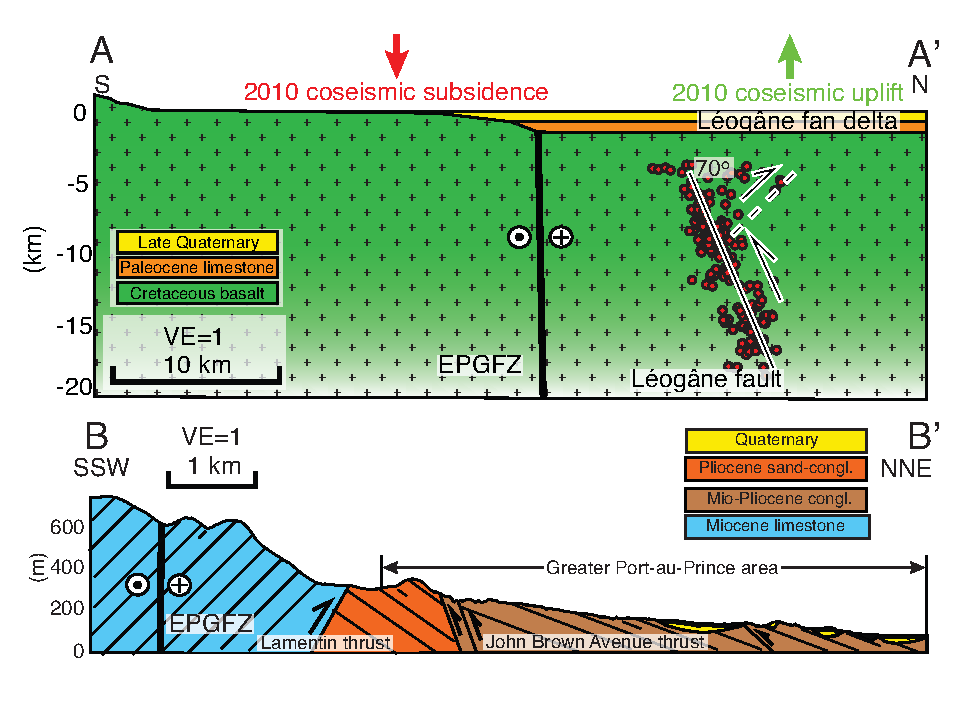
\includegraphics[width=\textwidth]{Haiti_figure3}
\caption{\textbf{Style of late Neogene, transpressional deformation in the northern belt along two transects shown in Figure~\ref{figure2}.} \textbf{A-A':} Aftershocks of the 2010 earthquake \citep{douilly2013crustal,douilly2015three} along the blind L\'eog\^ane thrust fault reveals conjugate reverse faults with the dominant slip occurring on the north-dipping fault. The red triangle indicates the location of L\'eog\^ane city. Coseismic uplift during the 2010 earthquake elevated the northern basinal area and depressed the mountains south of the EPGFZ. \textbf{B-B':} Cross section based on surface mapping \citep{massoni1955haiti,cox2011shear,mchugh2011offshore,saint2015seismotectonics} showing both north- and south-dipping reverse faults deforming Plio-Pleistocene sedimentary rocks.}
\label{figure3}
\end{figure}

\begin{figure}
\centering
\includegraphics[width=\textwidth]{Haiti_figure4}
\caption{\textbf{Geologic setting of Lake Azuey, Haiti.} \textbf{A:} To the south, the green-colored, brackish waters of Lake Azuey are bound by the EPGFZ which forms a sharp boundary with 2 km-high, folded limestone of Paleogene age that forms the smooth surfaces on the skyline. A fault strand of the EPGFZ marks the south edge of Lake Azuey while other parallel strands of the EPGFZ underlie the southern part of the lake as schematically shown. \textbf{B:} To the north of the lake folded, Plio-Pleistocene strata form the uplifted, 0 -- 30 m-high isthmus that separates Lake Azuey (15 m ASL) from Lake Enriquillo (46 m BSL) located 1 km to the east. Approximate locations of the EPGFZ and the Jimani thrust fault are shown.}
\label{figure4}
\end{figure}

\begin{figure}
\centering
\includegraphics[width=0.8\textwidth]{Haiti_figure5}
\caption{\textbf{Chirp sonar profiles showing the trace of the EPGFZ in the southern part of Lake Azuey and its relationship with a newly described thrust we have named the Jimani thrust.} Cross sections of A, B, C, and D are indicated in Figure~\ref{figure2}A. The EPGFZ beneath Lake Azuey forms a 250--500 m-wide zone that can be traced as a lineament to the east and west of Lake Azuey (Figure~\ref{figure2}). The green and red horizons represent two distinguish stratigraphic layers. The two strands of the EPGFZ are buried by 0.7 m of Holocene sediment and are extrapolated to be 270 years old since their last rupture when an average sedimentation rate of 2.6 mm/yr based on cores from Lake Enriquillo is assumed. Folds associate with the Jimani thrust are interpreted as fault propagation folds above northeast-dipping thrust faults. \textbf{E:} Cross section based on both sonar survey and the surface mapping \citep{mann1991overview} showing north- and south-dipping, reverse faults deforming Plio-Pleistocene sedimentary rocks.}
\label{figure5}
\end{figure}

\begin{figure}
\centering
\includegraphics[width=\textwidth]{Haiti_figure6}
\caption{\textbf{Structure of the EPGFZ in eastern Haiti and western-most Dominican Republic.} \textbf{A:} Structural map of Lakes Azuey (surface 15 m ASL) and Lake Enriquillo (surface 46 m BSL) are presently separated by a shallow sill 30 m ASL in the isthmus near the town of Jimani. \textbf{B:} Comparison of two Chirp lines from Lake Enriquillo by \citet{rios2013holocene} (3 km-long Line L19) and from our study of Lake Azuey (4 km-long Line B6). Chirp profiles from both lakes show similar sequences. Ages of units are known from Lake Enriquillo through both exposures around the sub-sea level lake and from lake coring by \citet{rios2013holocene}.}
\label{figure6}
\end{figure}

\begin{figure}
\centering
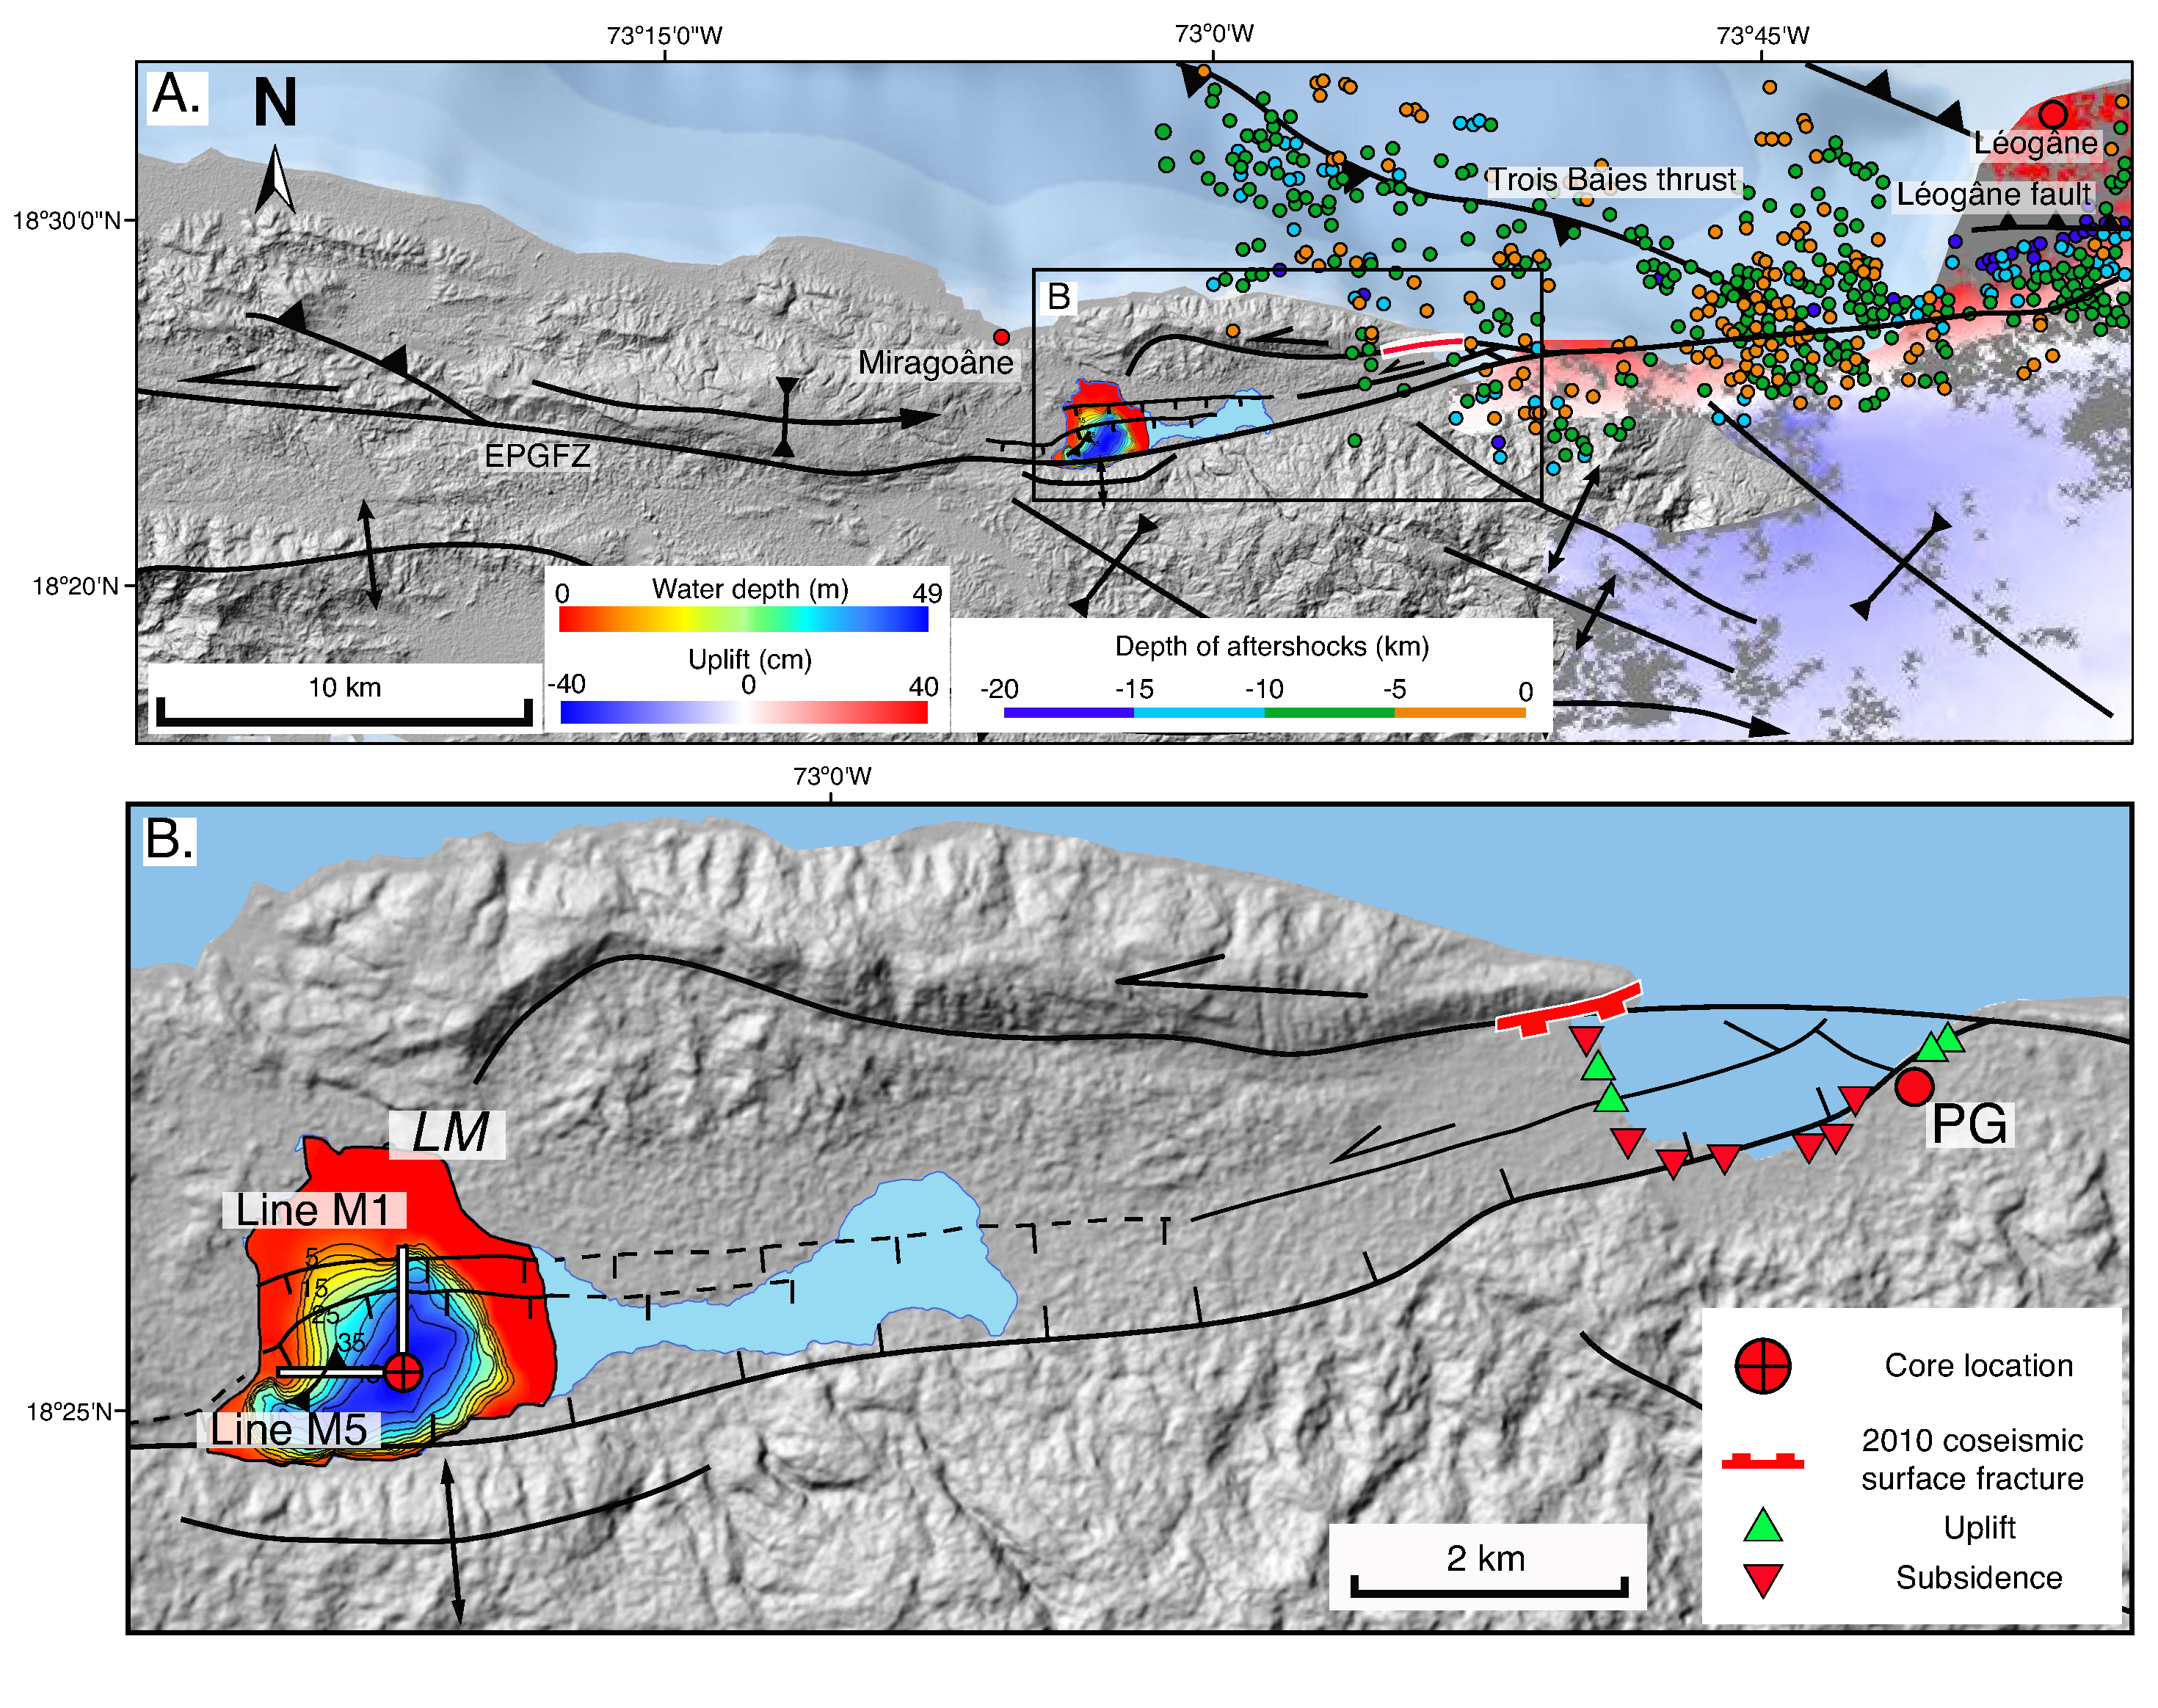
\includegraphics[width=\textwidth]{Haiti_figure7}
\caption{\textbf{Structure and 2010 coseismic surface deformation of the western segments of the EPGFZ.} \textbf{A:} Fault map \citep{prentice2010seismic,cowgill2012interactive} and map of 2010 aftershocks \citep{douilly2013crustal} in Mirago\^ane-L\'eog\^ane region overlain with an InSAR image (courtesy of Eric Fielding at JPL) \citep{hayes2010complex}. \textbf{B:} Zoom of the area of Petit Goave and Lake Mirago\^ane showing the structure and bathymetry of the 14 km\textsuperscript{2}, pull-apart basin underlying Lake Mirago\^ane during this study and details of the 2010 surface fracturing and coseismic subsidence in the Petit Go\^ave Bay \citep{prentice2010seismic,hornbach2010high}. \textbf{LM} = Lake Mirago\^ane; \textbf{PG} = Petit Go\^ave.}
\label{figure7}
\end{figure}

\begin{figure}
\centering
\includegraphics[width=\textwidth]{Haiti_figure8.pdf}
\caption{\textbf{Geologic setting and sonar profiles from Lake Mirago\^ane.} \textbf{A:} View looking south across the 12 km-wide and 42.8 m deep, freshwater lake. The 2 km-high, ridge along the southern edge of the lake is the cumulative topographic scarp associated with the southernmost strand of the EPGFZ. The 7 m-long core was taken by \citet{higuera199910}, but was not collected from the deepest part of the lake. \textbf{B:} North-south trending line M1 (location shown on Figure~\ref{figure7}B). \textbf{C:} East-west trending line M5 (location shown on Figure~\ref{figure7}B). In the lines shown in \textbf{B} and \textbf{C}, the strands of the EPGFZ are both buried by 0.5 m of sediment.}
\label{figure8}
\end{figure}

\begin{figure}
\centering
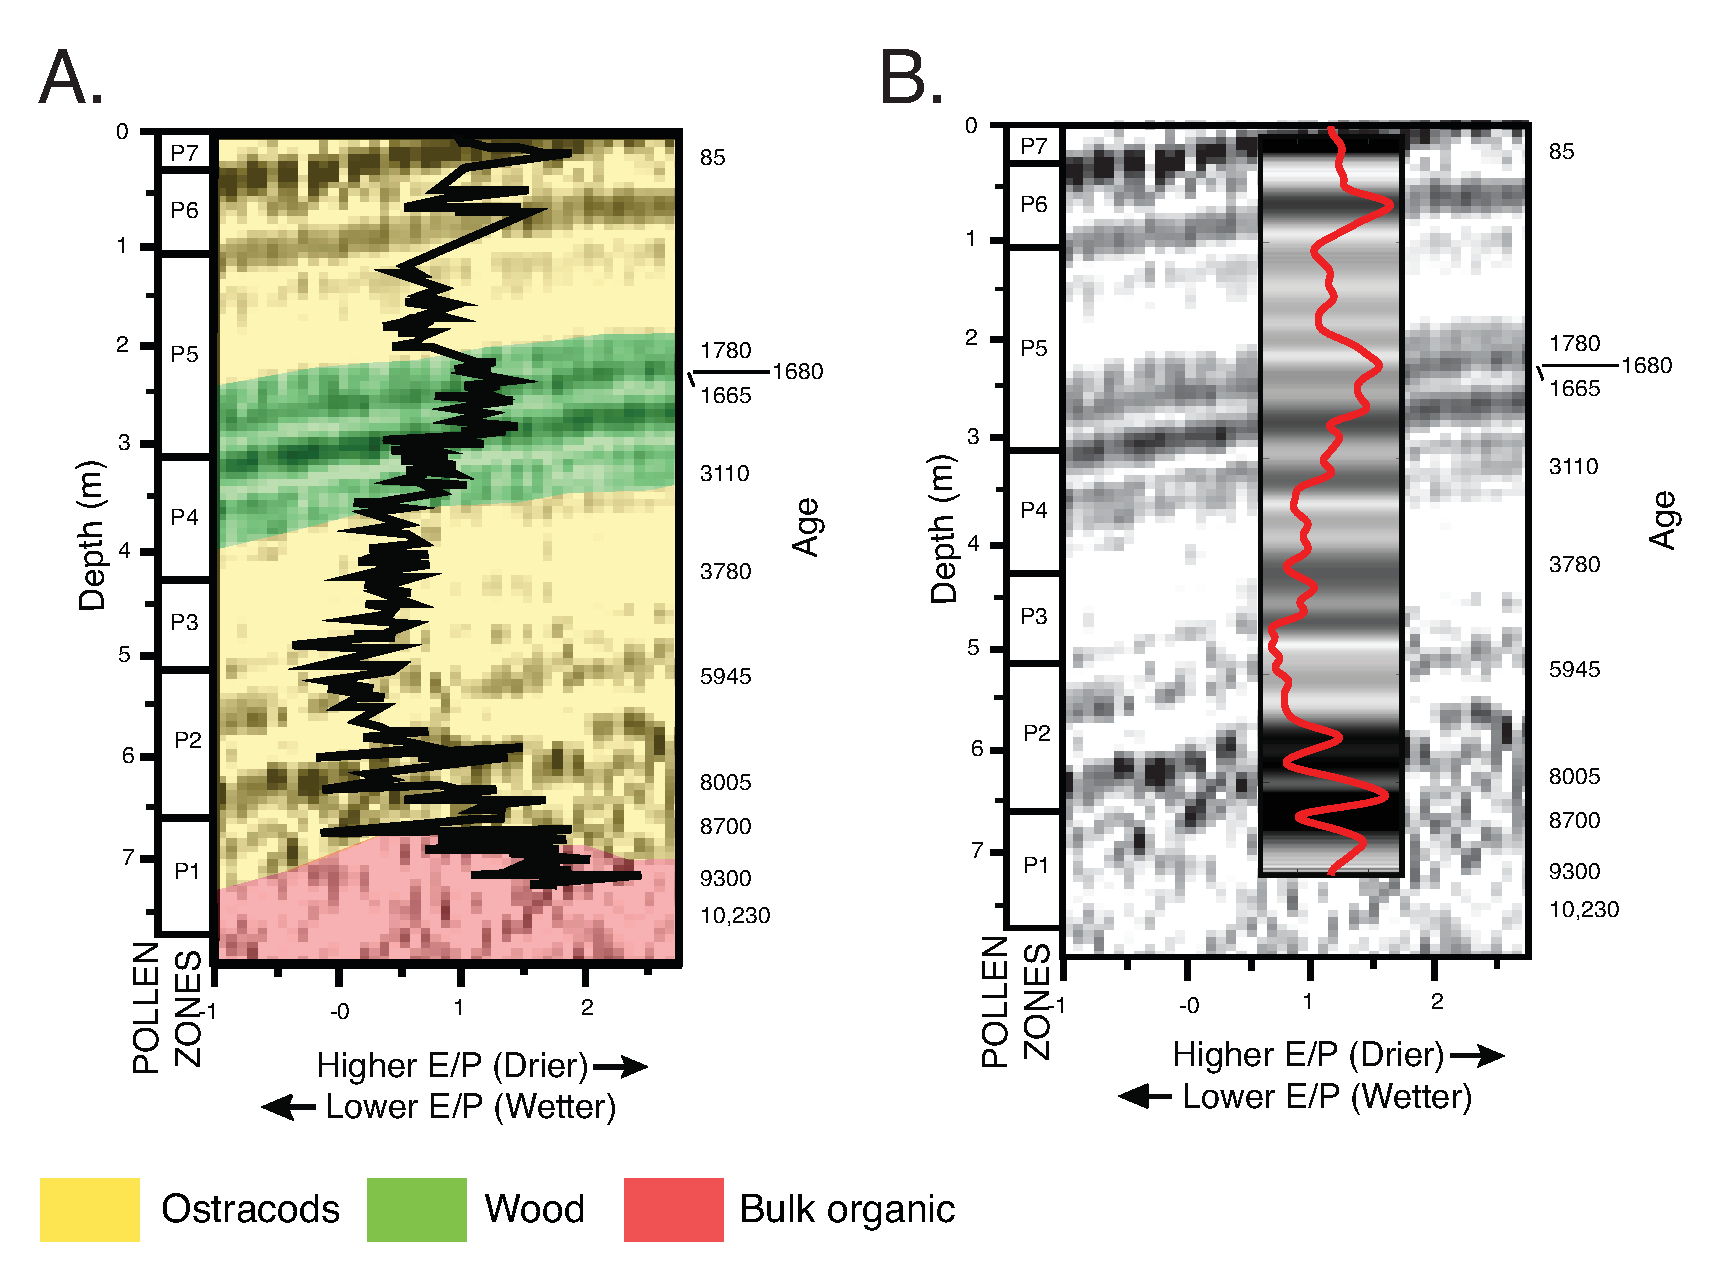
\includegraphics[width=\textwidth]{Haiti_figure9}
\caption{\textbf{Core data from Lake Mirago\^ane.} \textbf{A:} Tie between chirp sonar and core with radiocarbon age control back to 10,230 years BP. \citep{higuera199910} Cyclicity is related to changes in lithology related to alternating wet and dry periods as shown. Yellow areas are shallow marine to freshwater and green areas contain wood debris and may mark a period when the lake was dry. \textbf{B:} Low-pass filtered E/P log (red) and the synthetic sonar profile generated from the low-pass filtered E/P log used as an acoustic impedance. The chirp sonar profiles are from the location of the red bar in the Figure~\ref{figure8}B, C.}
\label{figure9}
\end{figure}

\begin{figure}
\centering
\includegraphics[width=\textwidth]{Haiti_figure10}
\caption{\textbf{Schematic diagram of the conjugate-thrust-fault model for the 10--15 km-wide belt of transpressional deformation along the northern edge of the EPGFZ. A:} Three-dimensional block diagram showing the structural, aftershocks, and the late Holocene strain partitioning in a 40-km-wide zone along a 120 km-long segment of the EPGFZ. Black arrows show the southwest direction of the GPS vectors relative to the Caribbean plate \citep{calais2010transpressional}. The 2010 InSAR-derived surface deformation map (provided by Eric Fielding at JPL) \citep{hayes2010complex} shows a large component of shortening accommodated on a 40 km-wide zone of oblique thrusts and folds north of the EPGFZ. Aftershock pattern shown in the cross section show that the northeastward dip of the \textit{en~echelon}. L\'eog\^ane thrust adjacent to the EPGFZ uplifted the topographically-lower, basinal area to the north of the EPGFZ and depressed the mountainous area to the south of the EPGFZ. The alternating dip of the \textit{en~echelon} thrusts is related to their origin as conjugate thrust faults in a highly transpressional setting. \textbf{PaP} = Port-au-Prince; \textbf{PG} = Petit Goave; \textbf{LA} = Lake Azuey; \textbf{LM} = Lake Mirago\^ane-L\'eog\^ane; \textbf{JF} = Jimani thrust fault; \textbf{DT} = Dumay thrust; \textbf{PFZ} = Port-au-Prince fault zone; \textbf{LMF} = Lamartin thrust fault; \textbf{TBF} = Trois Baies thrust fault; \textbf{LF} = L\'eog\^ane fault. \textbf{B:} Schematic diagram, modified from \citet{sibson2012reverse}, of the conjugate thrust faults.}
\label{figure10}
\end{figure}

\begin{figure}
\centering
\includegraphics[width=\textwidth]{Haiti_figure11}
\caption{\textbf{Structural map of the southern San Francisco Bay region, the co-seismic elevation and the aftershock cross-section of 1989 $M_w$ 6.9  Loma Prieta earthquake.} The selected GPS vectors relative to a fixed North America plate are from \citet{UNAVCO2009}. The coseismic elevation change and aftershock cross-section are modified from \citet{marshall1991faulting}. \textbf{SAF}: San Andreas Fault; \textbf{SF}: Sargent Fault. Aftershock pattern in the cross-section shows that the southwest dip of the \textit{en~echelon} thrust adjacent to the San Andreas fault uplifted the topographically-lower basinal area and depressed the mountainous area to the northeast of the San Andreas fault.}
\label{figure11}
\end{figure}

\end{document}
